\subsubsubsubsection{IssueDebitNote Function}

\begin{enumerate}

\item Profile

\begin{enumerate}

\item Description

The IssueDebitNote function is used to create the DebitNote Object by the Provider Node. It uses the POST /debitNotes method.
The DebitNote object is used for short-term billing of computing resource usage between a Provider node and a Requestor node.
 
\item Side

Provider

\end{enumerate}

\item Request

\begin{enumerate}

\item Input

\begin{tcolorbox}[boxrule=0pt, frame empty]
\begin{verbatim}

No parameters

\end{verbatim}
\end{tcolorbox}

Object

\begin{tcolorbox}[boxrule=0pt, frame empty]
\begin{verbatim}

{
  "activityId": "string",
  "totalAmountDue": "string",
  "usageCounterVector": {},
  "paymentDueDate": "YYYY-MM-DDThh:mm:ss.sssZ"
}

\end{verbatim}
\end{tcolorbox}

\begin{table}[H]
\footnotesize

\begin{center}
\begin{tabular}{|p{3cm}|l|p{3cm}|p{3cm}|p{4cm}|} 
\hline
\rowcolor{lightgray}	Name	& MO.	& Type	& Example & 	Description \\
\hline

activityId				& M	& 	string				&								&	Activity Identifier \\ 
\hline

totalAmountDue			& M	& 	string				&								&	Total Amount Due \\ 
\hline

usageCounterVector		& M & 	json				&								&	Usage Counter Vector \\
\hline

paymentDueDate			& M &	string(\$date-time)	&	YYYY-MM-DDThh:mm:ss.sssZ	&	Payment Due Date \\
\hline

\end{tabular}
\end{center}
\end{table}


\item REST Method

\begin{tcolorbox}[boxrule=0pt, frame empty]
\begin{verbatim} 

POST /debitNotes

\end{verbatim}
\end{tcolorbox}

\end{enumerate}

\item Response

\begin{table}[H]
\footnotesize

\begin{center}
\begin{tabular}{|c|l|} 
\hline
\rowcolor{lightgray}	Code 		& 	Description \\
\hline
201	 		&	OK \\
\hline
400			&	(400) Bad request \\
\hline
401			&	(401) Authorization information is missing or invalid. \\
\hline
500			&	(500) Server error. \\
\hline
\end{tabular}
\end{center}
\end{table}

\item Result

\begin{tcolorbox}[boxrule=0pt, frame empty]
\begin{verbatim}

{
  "debitNoteId": "string",
  "issuerId": "string",
  "recipientId": "string",
  "payeeAddr": "string",
  "payerAddr": "string",
  "paymentPlatform": "string",
  "previousDebitNoteId": "string",
  "timestamp": "YYYY-MM-DDThh:mm:ss.sss",
  "agreementId": "string",
  "activityId": "string",
  "totalAmountDue": "string",
  "usageCounterVector": {},
  "paymentDueDate": "YYYY-MM-DDThh:mm:ss.sssZ",
  "status": "ISSUED"
}

\end{verbatim}
\end{tcolorbox}

\begin{table}[H]
\footnotesize

\begin{center}
\begin{tabular}{|p{3cm}|l|p{3cm}|p{3cm}|p{4cm}|} 
\hline
\rowcolor{lightgray}	Name	& MO.	& Type	& Example & 	Description \\
\hline

debitNoteId				&	&	string				&																		&	Debit Note Identifier \\
\hline   

issuerId				&	&	string				&																		&	Issuer Identifier \\
\hline   
  
recipientId				&	&	string				&																		&	Recipient Identifier \\
\hline   

payeeAddr				&	&	string				&																		&	Payee Address \\
\hline   
  
payerAddr				&	&	string				&																		&	Payer Address \\
\hline
   
paymentPlatform			&	&	object(string)		&																		&	Payment Platform Object \\
\hline

previousDebitNoteId		&	&	string				&																		& 	Last Debit Note Id \\
\hline

timestamp				&   &	string(\$date-time)	&	YYYY-MM-DDThh:mm:ss.sssZ											&	Time of ? \\
\hline

agreementId				& 	& 	string				&																		&	Agreement Identifier \\ 
\hline

activityId				& 	& 	string				&																		&	Activity Identifier \\ 
\hline

totalAmountDue			& 	& 	string				&																		&	Total Amount Due \\ 
\hline

usageCounterVector		&   & 	json				&																		&	Usage Counter Vector \\
\hline

paymentDueDate			&   &	string(\$date-time)	&	YYYY-MM-DDThh:mm:ss.sssZ											&	Payment Due Date \\
\hline

status					&	&	string(enum)		&	[ISSUED, RECEIVED, ACCEPTED, REJECTED, FAILED, SETTLED, CANCELLED]	& 	Debit Note state \\	
\hline

\end{tabular}
\end{center}
\end{table}

\item Workflow

(Please see Figure ~\ref{fig:PCDN} on page ~\pageref{fig:PCDN}):

\begin{figure}[htbp]
    \centering
    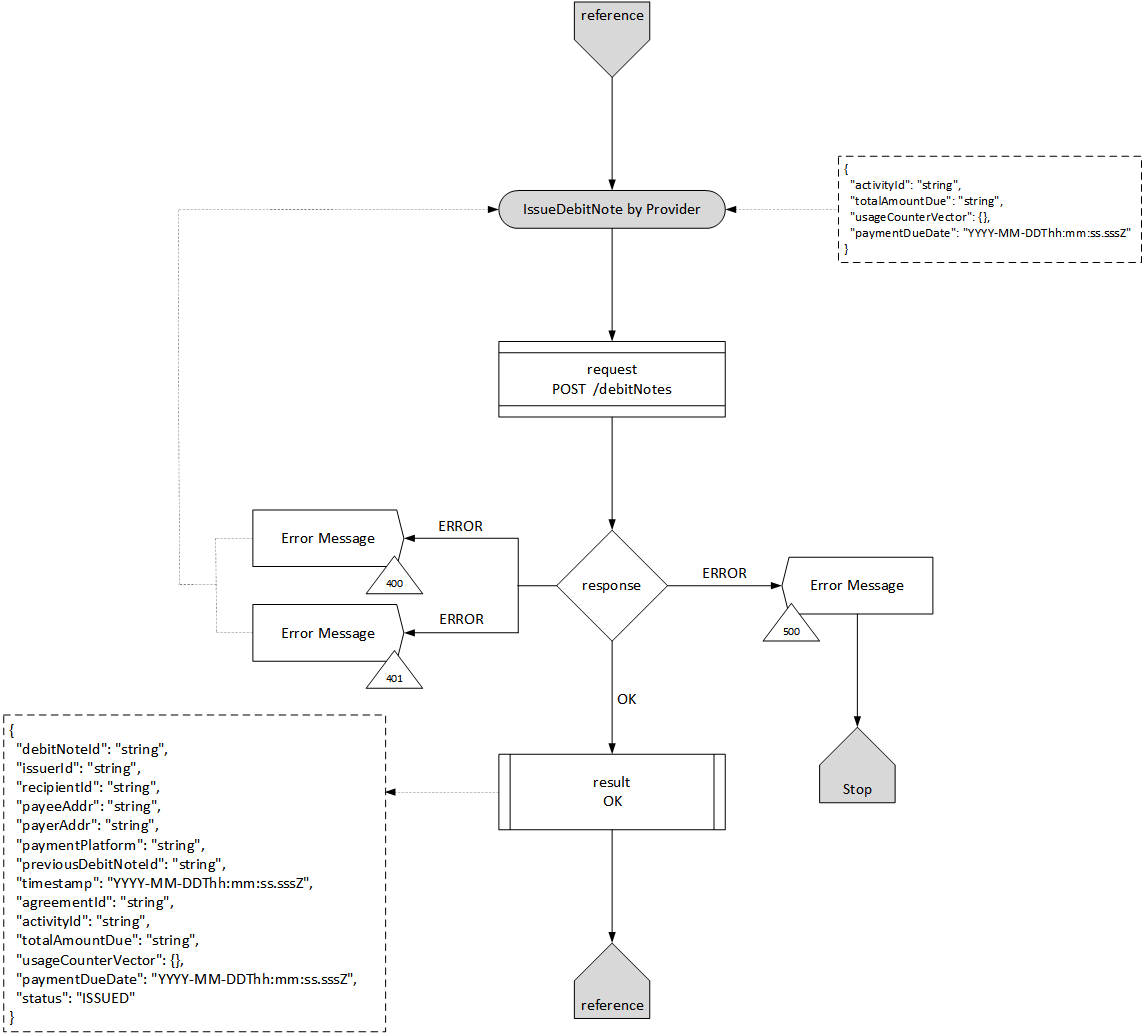
\includegraphics[width=12cm,height=12cm,angle=0]{./diag/Workflow/Payment/IssueDebitNote-P-Workflow.png}
    \caption{Provider Workflow Create Debit Note }
	\label{fig:PCDN}
\end{figure}


\end{enumerate}

\newpage

%% List Debit Notes

\subsubsubsubsection{ListDebitNotes Function}

\begin{enumerate}

\item Profile

\begin{enumerate}

\item Description

The ListDebitNotes function is used to get the DebitNote Objects by the Provider Node and Requestor Node. 
It uses the GET /debitNotes method.
 
\item Side

Both

\end{enumerate}

\item Request

\begin{enumerate}

\item Input

\begin{tcolorbox}[boxrule=0pt, frame empty]
\begin{verbatim}

afterTimestamp
maxItems

\end{verbatim}
\end{tcolorbox}

%Object
%\begin{tcolorbox}[boxrule=0pt, frame empty]
%\begin{verbatim}
%{
%  "activityId": "string",
%  "totalAmountDue": "string",
%  "usageCounterVector": {},
%  "paymentDueDate": "YYYY-MM-DDThh:mm:ss.sssZ"
%}
%\end{verbatim}
%\end{tcolorbox}

\begin{table}[H]
\footnotesize

\begin{center}
\begin{tabular}{|p{3cm}|l|p{3cm}|p{3cm}|p{4cm}|} 
\hline
\rowcolor{lightgray}	Name	& MO.	& Type	& Example & 	Description \\
\hline

maxItems				& O	& 	integer(\$int32)	&	10							&	Maximum number of items that server should return at once. \\ 
\hline

afterTimestamp			& O &	string(\$date-time)	&	YYYY-MM-DDThh:mm:ss.sssZ	&	Apply only to records created later than the specified timestamp \\
\hline

\end{tabular}
\end{center}
\end{table}


\item REST Method

\begin{tcolorbox}[boxrule=0pt, frame empty]
\begin{verbatim} 

GET /debitNotes

\end{verbatim}
\end{tcolorbox}

\end{enumerate}

\item Response

\begin{table}[H]
\footnotesize
\begin{center}
\begin{tabular}{|c|l|} 
\hline
\rowcolor{lightgray}	Code 		& 	Description \\
\hline
201	 		&	OK \\
\hline
401			&	(401) Authorization information is missing or invalid. \\
\hline
500			&	(500) Server error. \\
\hline
\end{tabular}
\end{center}
\end{table}

\item Result

\begin{tcolorbox}[boxrule=0pt, frame empty]
\begin{verbatim}

[
	{
		"debitNoteId": "string",
		"issuerId": "string",
		"recipientId": "string",
		"payeeAddr": "string",
		"payerAddr": "string",
		"paymentPlatform": "string",
		"previousDebitNoteId": "string",
		"timestamp": "YYYY-MM-DDThh:mm:ss.sss",
		"agreementId": "string",
		"activityId": "string",
		"totalAmountDue": "string",
		"usageCounterVector": {},
		"paymentDueDate": "YYYY-MM-DDThh:mm:ss.sssZ",
		"status": "ISSUED"
	}
]

\end{verbatim}
\end{tcolorbox}

\begin{table}[H]
\footnotesize

\begin{center}
\begin{tabular}{|p{3cm}|l|p{3cm}|p{3cm}|p{4cm}|} 
\hline
\rowcolor{lightgray}	Name	& MO.	& Type	& Example & 	Description \\
\hline

debitNoteId				&	&	string				&																		&	Debit Note Identifier \\
\hline   

issuerId				&	&	string				&																		&	Issuer Identifier \\
\hline   
  
recipientId				&	&	string				&																		&	Recipient Identifier \\
\hline   

payeeAddr				&	&	string				&																		&	Payee Address \\
\hline   
  
payerAddr				&	&	string				&																		&	Payer Address \\
\hline
   
paymentPlatform			&	&	object(string)		&																		&	Payment Platform Object \\
\hline

previousDebitNoteId		&	&	string				&																		& 	Last Debit Note Id \\
\hline

timestamp				&   &	string(\$date-time)	&	YYYY-MM-DDThh:mm:ss.sssZ											&	Time of ? \\
\hline

agreementId				& 	& 	string				&																		&	Agreement Identifier \\ 
\hline

activityId				& 	& 	string				&																		&	Activity Identifier \\ 
\hline

totalAmountDue			& 	& 	string				&																		&	Total Amount Due \\ 
\hline

usageCounterVector		&   & 	json				&																		&	Usage Counter Vector \\
\hline

paymentDueDate			&   &	string(\$date-time)	&	YYYY-MM-DDThh:mm:ss.sssZ											&	Payment Due Date \\
\hline

status					&	&	string(enum)		&	[ISSUED, RECEIVED, ACCEPTED, REJECTED, FAILED, SETTLED, CANCELLED]	& 	Debit Note state \\	
\hline

\end{tabular}
\end{center}
\end{table}

\item Workflow

(Please see Figure ~\ref{fig:BLDN} on page ~\pageref{fig:BLDN}):

\begin{figure}[htbp]
    \centering
    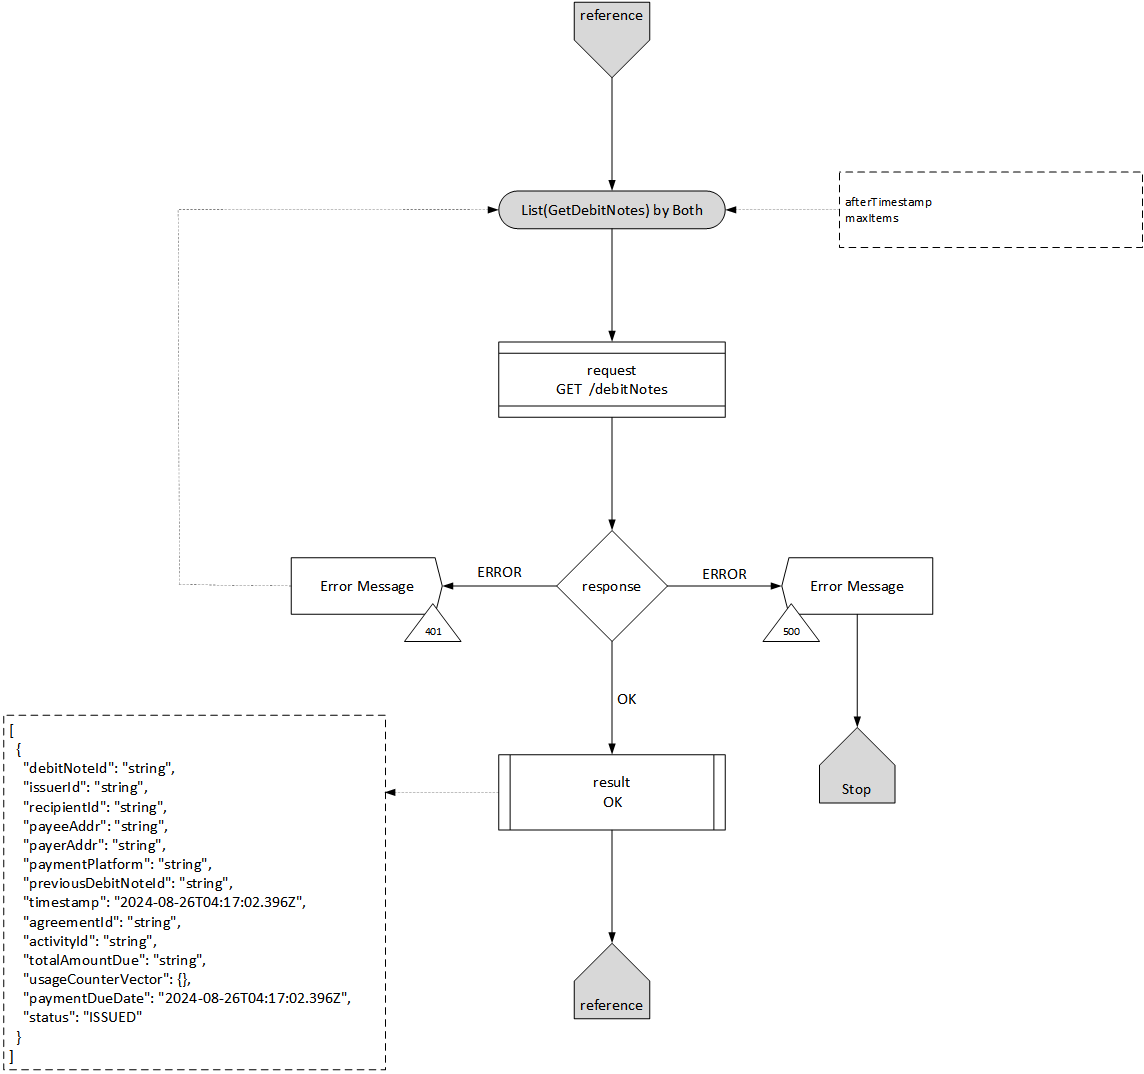
\includegraphics[width=12cm,height=12cm,angle=0]{./diag/Workflow/Payment/List(GetDebitNotes)-B-Workflow.png}
    \caption{Both Workflow List Debit Notes }
	\label{fig:BLDN}
\end{figure}


\end{enumerate}

\newpage

%% Get Debit Notes

\subsubsubsubsection{GetDebitNote Function}

\begin{enumerate}

\item Profile

\begin{enumerate}

\item Description

The GetDebitNote function is used to get the DebitNote Object by the Provider Node and Requestor Node. 
It uses the GET /debitNotes/\{debitNoteId\} method.
 
\item Side

Both

\end{enumerate}

\item Request

\begin{enumerate}

\item Input

\begin{tcolorbox}[boxrule=0pt, frame empty]
\begin{verbatim}

debitNoteId

\end{verbatim}
\end{tcolorbox}

%Object
%\begin{tcolorbox}[boxrule=0pt, frame empty]
%\begin{verbatim}
%{
%  "activityId": "string",
%  "totalAmountDue": "string",
%  "usageCounterVector": {},
%  "paymentDueDate": "YYYY-MM-DDThh:mm:ss.sssZ"
%}
%\end{verbatim}
%\end{tcolorbox}

\begin{table}[H]
\footnotesize

\begin{center}
\begin{tabular}{|p{3cm}|l|p{3cm}|p{3cm}|p{4cm}|} 
\hline
\rowcolor{lightgray}	Name	& MO.	& Type	& Example & 	Description \\
\hline

debitNoteId				& M	& 	string				&								&	Debit Note Identifier \\ 
\hline

%afterTimestamp			& O &	string(\$date-time)	&	YYYY-MM-DDThh:mm:ss.sssZ	&	Apply only to records created later than the specified timestamp \\
%\hline

\end{tabular}
\end{center}
\end{table}


\item REST Method

\begin{tcolorbox}[boxrule=0pt, frame empty]
\begin{verbatim} 

GET /debitNotes/{debitNoteId}

\end{verbatim}
\end{tcolorbox}

\end{enumerate}

\item Response

\begin{table}[H]
\footnotesize

\begin{center}
\begin{tabular}{|c|l|} 
\hline
\rowcolor{lightgray}	Code 		& 	Description \\
\hline
201	 		&	OK \\
\hline
401			&	(401) Authorization information is missing or invalid. \\
\hline
404			&	(404) The specified resource was not found \\
\hline
500			&	(500) Server error. \\
\hline
\end{tabular}
\end{center}

\end{table}

\item Result

\begin{tcolorbox}[boxrule=0pt, frame empty]
\begin{verbatim}


{
	"debitNoteId": "string",
	"issuerId": "string",
	"recipientId": "string",
	"payeeAddr": "string",
	"payerAddr": "string",
	"paymentPlatform": "string",
	"previousDebitNoteId": "string",
	"timestamp": "YYYY-MM-DDThh:mm:ss.sss",
	"agreementId": "string",
	"activityId": "string",
	"totalAmountDue": "string",
	"usageCounterVector": {},
	"paymentDueDate": "YYYY-MM-DDThh:mm:ss.sssZ",
	"status": "ISSUED"
}


\end{verbatim}
\end{tcolorbox}

\begin{table}
\footnotesize

\begin{center}
\begin{tabular}{|p{3cm}|l|p{3cm}|p{3cm}|p{4cm}|} 
\hline
\rowcolor{lightgray}	Name	& MO.	& Type	& Example & 	Description \\
\hline

debitNoteId				&	&	string				&																		&	Debit Note Identifier \\
\hline   

issuerId				&	&	string				&																		&	Issuer Identifier \\
\hline   
  
recipientId				&	&	string				&																		&	Recipient Identifier \\
\hline   

payeeAddr				&	&	string				&																		&	Payee Address \\
\hline   
  
payerAddr				&	&	string				&																		&	Payer Address \\
\hline
   
paymentPlatform			&	&	object(string)		&																		&	Payment Platform Object \\
\hline

previousDebitNoteId		&	&	string				&																		& 	Last Debit Note Id \\
\hline

timestamp				&   &	string(\$date-time)	&	YYYY-MM-DDThh:mm:ss.sssZ											&	Time of ? \\
\hline

agreementId				& 	& 	string				&																		&	Agreement Identifier \\ 
\hline

activityId				& 	& 	string				&																		&	Activity Identifier \\ 
\hline

totalAmountDue			& 	& 	string				&																		&	Total Amount Due \\ 
\hline

usageCounterVector		&   & 	json				&																		&	Usage Counter Vector \\
\hline

paymentDueDate			&   &	string(\$date-time)	&	YYYY-MM-DDThh:mm:ss.sssZ											&	Payment Due Date \\
\hline

status					&	&	string(enum)		&	[ISSUED, RECEIVED, ACCEPTED, REJECTED, FAILED, SETTLED, CANCELLED]	& 	Debit Note state \\	
\hline

\end{tabular}
\end{center}
\end{table}

\item Workflow

(Please see Figure ~\ref{fig:BGDN} on page ~\pageref{fig:BGDN}):

\begin{figure}[htbp]
    \centering
    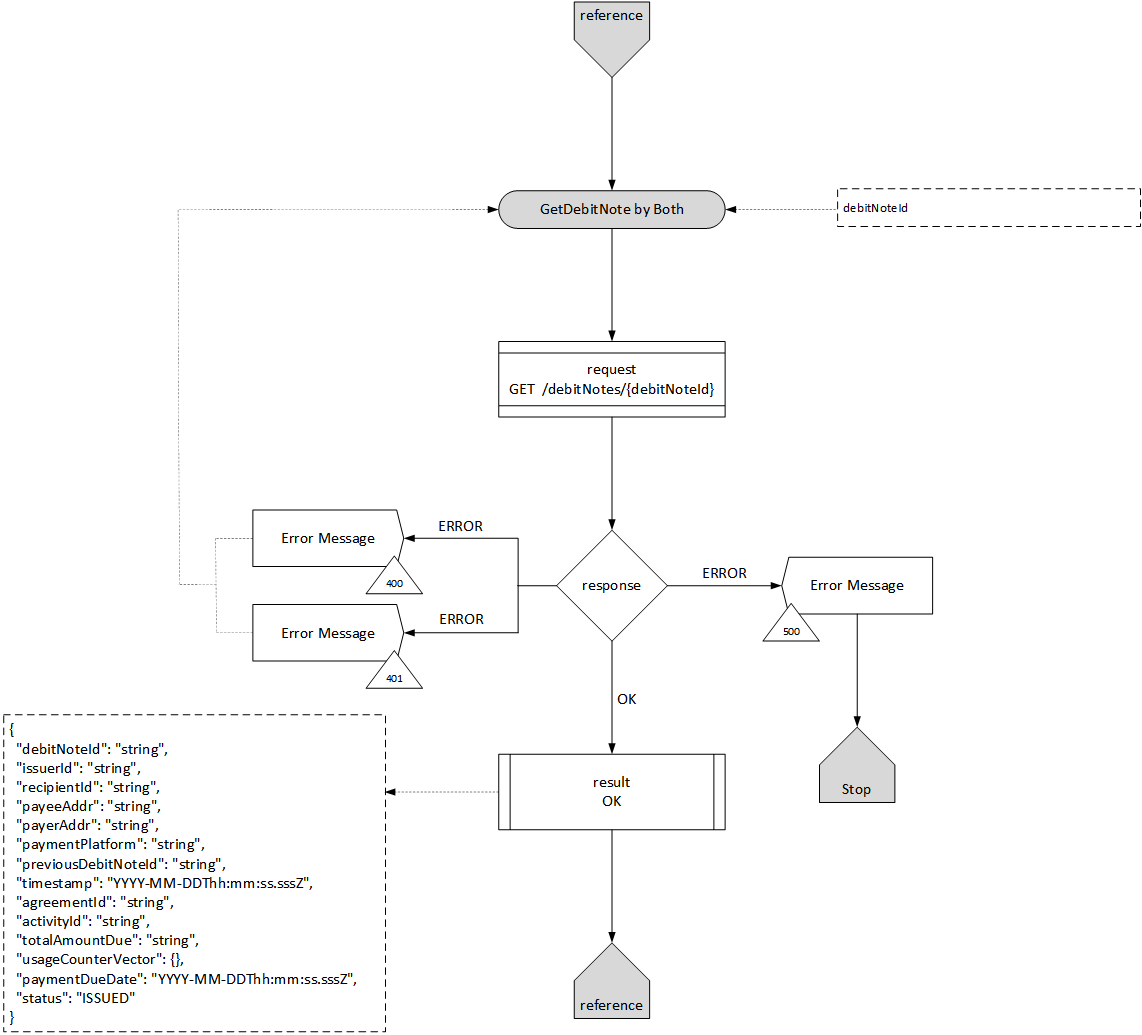
\includegraphics[width=12cm,height=12cm,angle=0]{./diag/Workflow/Payment/GetDebitNote-B-Workflow.png}
    \caption{Both Workflow Get Debit Note }
	\label{fig:BGDN}
\end{figure}


\end{enumerate}

\newpage

%% DebitNoteEvents

\subsubsubsubsection{CollectDebitNoteInvoiceEvent Function}

\begin{enumerate}

\item Profile

\begin{enumerate}

\item Description

The CollectDebitNoteInvoiceEvent function is used to get the DebitNote events by the Provider Node and Requestor Node. 
It uses the GET /debitNoteEvents method.
 
\item Side

Both

\end{enumerate}

\item Request

\begin{enumerate}

\item Input

\begin{tcolorbox}[boxrule=0pt, frame empty]
\begin{verbatim}

timeout
afterTimestamp
maxEvents
appSessionId

\end{verbatim}
\end{tcolorbox}

%Object
%\begin{tcolorbox}[boxrule=0pt, frame empty]
%\begin{verbatim}
%{
%  "activityId": "string",
%  "totalAmountDue": "string",
%  "usageCounterVector": {},
%  "paymentDueDate": "YYYY-MM-DDThh:mm:ss.sssZ"
%}
%\end{verbatim}
%\end{tcolorbox}

\begin{table}[H]
\footnotesize

\begin{center}
\begin{tabular}{|p{3cm}|l|p{3cm}|p{3cm}|p{4cm}|} 
\hline
\rowcolor{lightgray}	Name	& MO.	& Type	& Example & 	Description \\
\hline

timeout					& O	& 	number(\$float)		&	5							&	Timeout used in long-polling calls (in seconds). 
																						How many seconds server should wait for response containing new events 
																						(0.0 means it should return immediately if there are no events) \\ 
\hline

afterTimestamp			& O &	string(\$date-time)	&	YYYY-MM-DDThh:mm:ss.sssZ	&	Apply only to records created later than the specified timestamp \\
\hline

maxEvents				& O & 	integer(\$int32)	&	10							&	Maximum number of events that server should return at once. \\
\hline

appSessionId			& O &	string				&								&	A correlation/session identifier used for querying events related to 
																						an action where this appSessionId has been specified \\
\hline

\end{tabular}
\end{center}
\end{table}


\item REST Method

\begin{tcolorbox}[boxrule=0pt, frame empty]
\begin{verbatim} 

GET /debitNoteEvents

\end{verbatim}
\end{tcolorbox}

\end{enumerate}

\item Response

\begin{table}[H]
\footnotesize

\begin{center}
\begin{tabular}{|c|l|} 
\hline
\rowcolor{lightgray}	Code 		& 	Description \\
\hline
201	 		&	OK \\
\hline
401			&	(401) Authorization information is missing or invalid. \\
\hline
%404			&	(404) The specified resource was not found \\
%\hline
500			&	(500) Server error. \\
\hline
\end{tabular}
\end{center}

\end{table}

\item Result

\begin{tcolorbox}[boxrule=0pt, frame empty]
\begin{verbatim}

[
  {
    "eventType": "string",
    "eventDate": "YYYY-MM-DDThh:mm:ss.sssZ",
    "debitNoteId": "string"
  }
]


\end{verbatim}
\end{tcolorbox}

\begin{table}[H]
\footnotesize

\begin{center}
\begin{tabular}{|p{3cm}|l|p{3cm}|p{3cm}|p{4cm}|} 
\hline
\rowcolor{lightgray}	Name	& MO.	& Type	& Example & 	Description \\
\hline

debitNoteId				&	&	string				&																		&	Debit Note Identifier \\
\hline   

eventDate				&   &	string(\$date-time)	&	YYYY-MM-DDThh:mm:ss.sssZ											&	Event Date \\
\hline

eventType				&	&	string				&																		& 	Event Type \\	
\hline

\end{tabular}
\end{center}
\end{table}

\item Workflow

(Please see Figure ~\ref{fig:BGDNE} on page ~\pageref{fig:BGDNE}):

\begin{figure}[htbp]
    \centering
    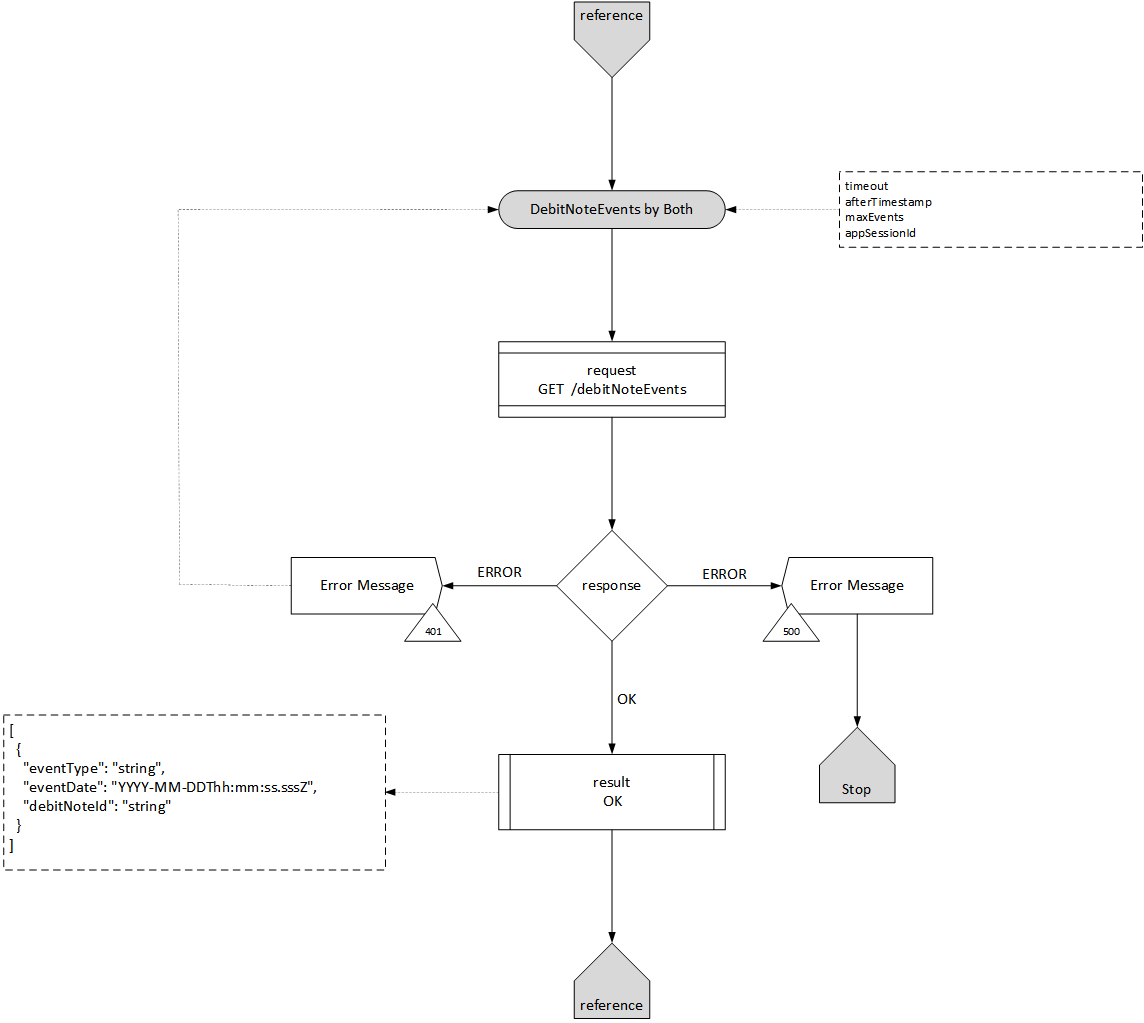
\includegraphics[width=12cm,height=12cm,angle=0]{./diag/Workflow/Payment/DebitNoteEvents-B-Workflow.png}
    \caption{Both Workflow Get Debit Note Events }
	\label{fig:BGDNE}
\end{figure}


\end{enumerate}

\newpage

% SendDebitNote 

\subsubsubsubsection{SendDebitNote Function}

\begin{enumerate}

\item Profile

\begin{enumerate}

\item Description

The SendDebitNote function is used to send the DebitNote Object from the Provider Node to the Requestor Node. 
It uses the POST /debitNotes/\{debitNoteId\}/send method.

\item Side

Provider

\end{enumerate}

\item Request

\begin{enumerate}

\item Input

\begin{tcolorbox}[boxrule=0pt, frame empty]
\begin{verbatim}

debitNoteId
timeout

\end{verbatim}
\end{tcolorbox}

%Object

%\begin{tcolorbox}[boxrule=0pt, frame empty]
%\begin{verbatim}

%{
%  "activityId": "string",
%  "totalAmountDue": "string",
%  "usageCounterVector": {},
%  "paymentDueDate": "YYYY-MM-DDThh:mm:ss.sssZ"
%}

%\end{verbatim}
%\end{tcolorbox}

\begin{table}[H]
\footnotesize

\begin{center}
\begin{tabular}{|p{3cm}|l|p{3cm}|p{3cm}|p{4cm}|} 
\hline
\rowcolor{lightgray}	Name	& MO.	& Type	& Example & 	Description \\
\hline

debitNoteId				& M	&	string				&								&	Debit Note Identifier \\
\hline   

timeout					& O &	number(\$float)		&	5							&	Timeout used in blocking calls waiting for eg. acknowledgement. 
																						How many seconds server should wait for response/acknowledgement 
																						of an action 
																						(0.0 means it should wait for other party's response indefinitely) \\
\hline

\end{tabular}
\end{center}
\end{table}


\item REST Method

\begin{tcolorbox}[boxrule=0pt, frame empty]
\begin{verbatim} 

POST /debitNotes/{debitNoteId}/send

\end{verbatim}
\end{tcolorbox}

\end{enumerate}

\item Response

\begin{table}[H]
\footnotesize

\begin{center}
\begin{tabular}{|c|l|} 
\hline
\rowcolor{lightgray}	Code 		& 	Description \\
\hline
200	 		&	OK \\
\hline
404			&	(404) The specified resource was not found. \\
\hline
401			&	(401) Authorization information is missing or invalid. \\
\hline
500			&	(500) Server error. \\
\hline
504			&	(504) Ack timeout. \\
\hline

\end{tabular}
\end{center}

\end{table}

\item Result

\begin{tcolorbox}[boxrule=0pt, frame empty]
\begin{verbatim}

As above

\end{verbatim}
\end{tcolorbox}

%\begin{table}[H]
%\footnotesize
%\begin{center}
%\begin{tabular}{|p{3cm}|l|p{3cm}|p{3cm}|p{4cm}|} 
%\hline
%\rowcolor{lightgray}	Name	& MO.	& Type	& Example & 	Description \\
%\hline	
%\end{tabular}
%\end{center}
%\end{table}

\item Workflow

(Please see Figure ~\ref{fig:PSDN} on page ~\pageref{fig:PSDN}):

\begin{figure}[htbp]
    \centering
    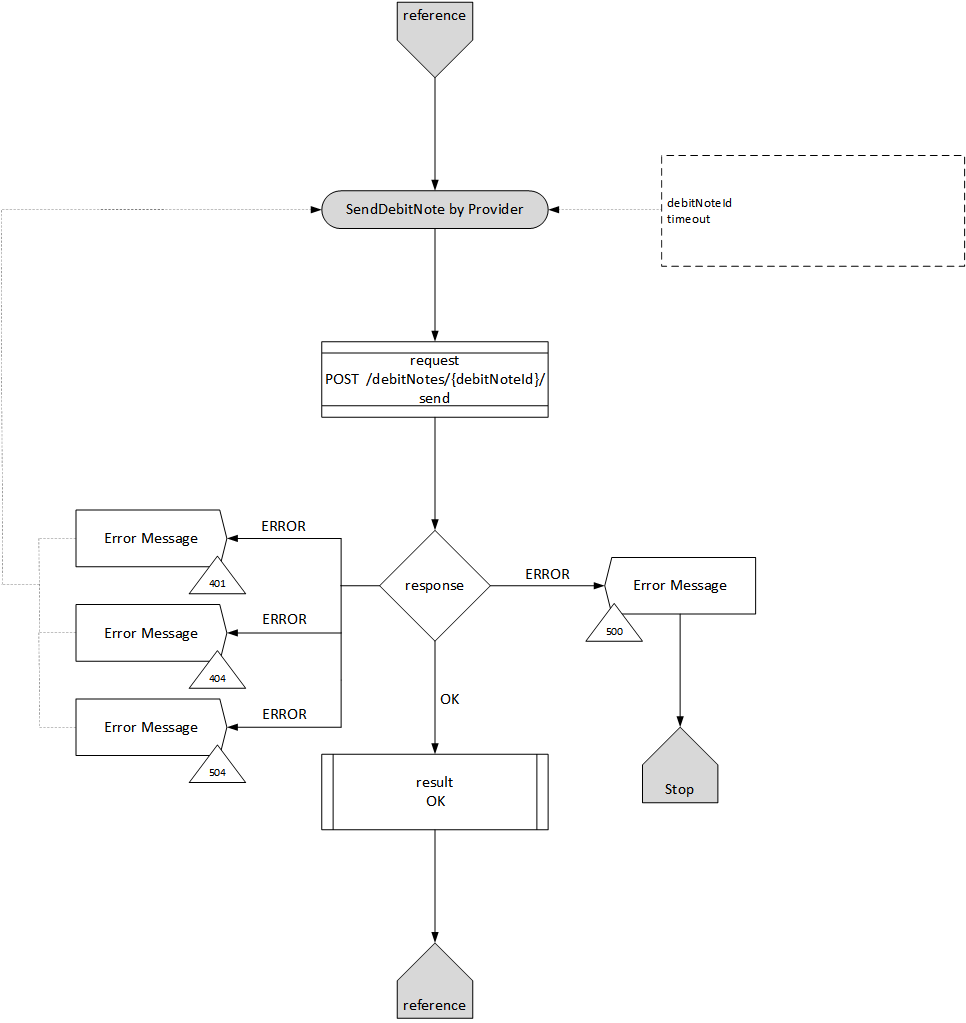
\includegraphics[width=12cm,height=12cm,angle=0]{./diag/Workflow/Payment/SendDebitNote-P-Workflow.png}
    \caption{Provider Workflow Send Debit Note }
	\label{fig:PSDN}
\end{figure}


\end{enumerate}

\newpage


% AcceptDebitNote 

\subsubsubsubsection{AcceptDebitNote Function}

\begin{enumerate}

\item Profile

\begin{enumerate}

\item Description

The AcceptDebitNote function is used to accept received the DebitNote Object by the Requestor Node. 
It uses the POST /debitNotes/\{debitNoteId\}/accept method.

\item Side

Requestor

\end{enumerate}

\item Request

\begin{enumerate}

\item Input

\begin{tcolorbox}[boxrule=0pt, frame empty]
\begin{verbatim}

debitNoteId
timeout

\end{verbatim}
\end{tcolorbox}

Object

\begin{tcolorbox}[boxrule=0pt, frame empty]
\begin{verbatim}

{
  "totalAmountAccepted": "string",
  "allocationId": "string",
  "autoAcceptTo": "string"
}

\end{verbatim}
\end{tcolorbox}

\begin{table}[H]
\footnotesize

\begin{center}
\begin{tabular}{|p{3cm}|l|p{3cm}|p{3cm}|p{4cm}|} 
\hline
\rowcolor{lightgray}	Name	& MO.	& Type	& Example & 	Description \\
\hline

debitNoteId				& M	&	string				&								&	Debit Note Identifier \\
\hline   

timeout					& O &	number(\$float)		&	5							&	Timeout used in blocking calls waiting for eg. acknowledgement. 
																						How many seconds server should wait for response/acknowledgement 
																						of an action 
																						(0.0 means it should wait for other party's response indefinitely) \\
\hline

totalAmountAccepted		& M &	string				&								&			\\
\hline

allocationId			& M &  	string				&								&			\\
\hline

autoAcceptTo 			& M & 	string				&								&			\\
\hline

\end{tabular}
\end{center}
\end{table}


\item REST Method

\begin{tcolorbox}[boxrule=0pt, frame empty]
\begin{verbatim} 

POST /debitNotes/{debitNoteId}/accept

\end{verbatim}
\end{tcolorbox}

\end{enumerate}

\item Response

\begin{table}[H]
\footnotesize

\begin{center}
\begin{tabular}{|c|l|} 
\hline
\rowcolor{lightgray}	Code 		& 	Description \\
\hline
200	 		&	OK \\
\hline
400			&	(400) Bad request \\
\hline
404			&	(404) The specified resource was not found. \\
\hline
401			&	(401) Authorization information is missing or invalid. \\
\hline
500			&	(500) Server error. \\
\hline
504			&	(504) Ack timeout. \\
\hline

\end{tabular}
\end{center}

\end{table}

\item Result

\begin{tcolorbox}[boxrule=0pt, frame empty]
\begin{verbatim}

As above

\end{verbatim}
\end{tcolorbox}

%\begin{table}
%\footnotesize
%\begin{center}
%\begin{tabular}{|p{3cm}|l|p{3cm}|p{3cm}|p{4cm}|} 
%\hline
%\rowcolor{lightgray}	Name	& MO.	& Type	& Example & 	Description \\
%\hline	
%\end{tabular}
%\end{center}
%\end{table}

\item Workflow

(Please see Figure ~\ref{fig:RADN} on page ~\pageref{fig:RADN}):

\begin{figure}[htbp]
    \centering
    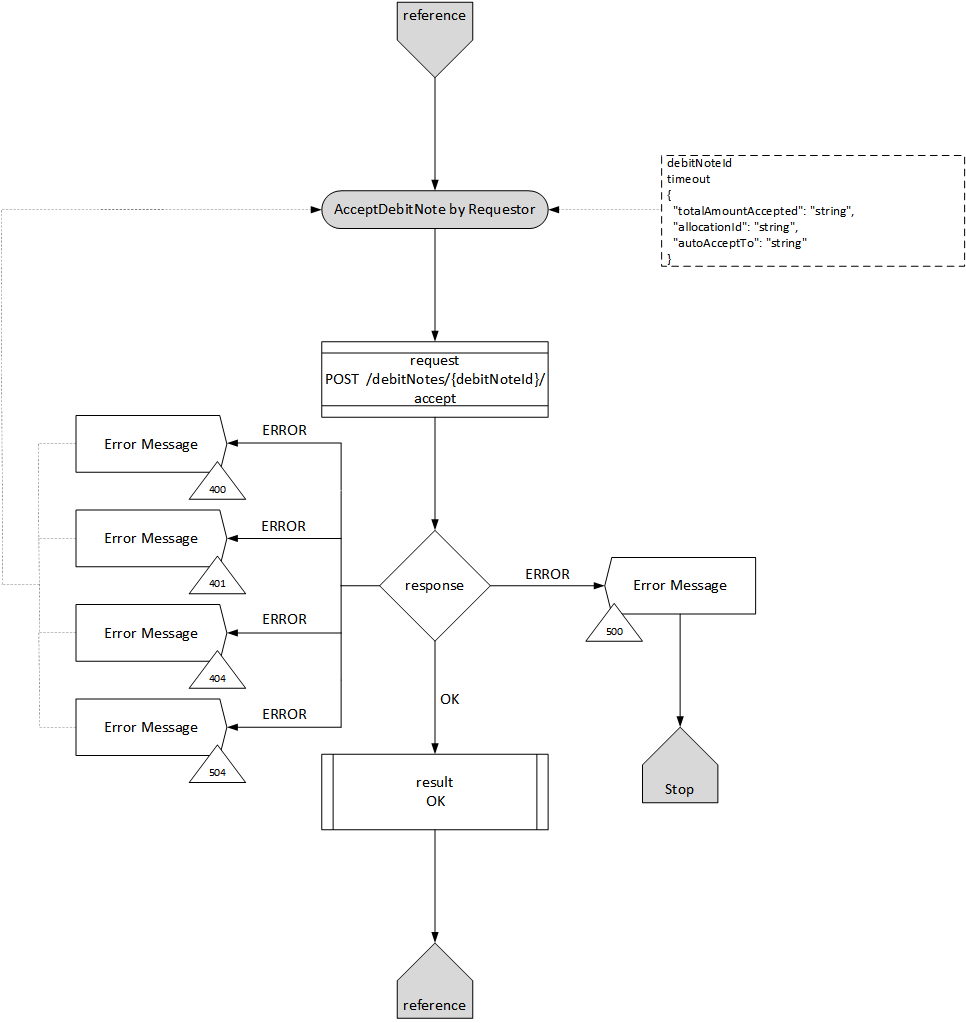
\includegraphics[width=12cm,height=12cm,angle=0]{./diag/Workflow/Payment/AcceptDebitNote-R-Workflow.png}
    \caption{Requestor Workflow Accept Debit Note }
	\label{fig:RADN}
\end{figure}


\end{enumerate}

\newpage

% RejectDebitNote  %%%

\subsubsubsubsection{RejectDebitNote Function}

\begin{enumerate}

\item Profile

\begin{enumerate}

\item Description

The RejectDebitNote function is used to reject received the DebitNote Object by the Requestor Node. 
It uses the POST /debitNotes/\{debitNoteId\}/reject method.

\item Side

Requestor

\end{enumerate}

\item Request

\begin{enumerate}

\item Input

\begin{tcolorbox}[boxrule=0pt, frame empty]
\begin{verbatim}

debitNoteId
timeout

\end{verbatim}
\end{tcolorbox}

Object

\begin{tcolorbox}[boxrule=0pt, frame empty]
\begin{verbatim}

{
  "rejectionReason": "UNSOLICITED_SERVICE",
  "totalAmountAccepted": "string",
  "message": "string"
}

\end{verbatim}
\end{tcolorbox}

\begin{table}[H]
\footnotesize

\begin{center}
\begin{tabular}{|p{3cm}|l|p{3cm}|p{3cm}|p{4cm}|} 
\hline
\rowcolor{lightgray}	Name	& MO.	& Type	& Example & 	Description \\
\hline

debitNoteId				& M	&	string				&								&	Debit Note Identifier \\
\hline   

timeout					& O &	number(\$float)		&	5							&	Timeout used in blocking calls waiting for eg. acknowledgement. 
																						How many seconds server should wait for response/acknowledgement 
																						of an action 
																						(0.0 means it should wait for other party's response indefinitely) \\
\hline

totalAmountAccepted		& M &	string				&								&			\\
\hline

message					& M &  	string				&								&			\\
\hline

rejectionReason 		& M & 	string(enum)		&	[UNSOLICITED\_SERVICE, BAD\_SERVICE, INCORRECT\_AMOUNT]	&	Possible reasons to reject a Debit Note		\\
\hline

\end{tabular}
\end{center}
\end{table}


\item REST Method

\begin{tcolorbox}[boxrule=0pt, frame empty]
\begin{verbatim} 

POST /debitNotes/{debitNoteId}/reject

\end{verbatim}
\end{tcolorbox}

\end{enumerate}

\item Response

\begin{table}[H]
\footnotesize

\begin{center}
\begin{tabular}{|c|l|} 
\hline
\rowcolor{lightgray}	Code 		& 	Description \\
\hline
200	 		&	OK \\
\hline
400			&	(400) Bad request \\
\hline
404			&	(404) The specified resource was not found. \\
\hline
401			&	(401) Authorization information is missing or invalid. \\
\hline
500			&	(500) Server error. \\
\hline
504			&	(504) Ack timeout. \\
\hline

\end{tabular}
\end{center}

\end{table}

\item Result

\begin{tcolorbox}[boxrule=0pt, frame empty]
\begin{verbatim}

As above

\end{verbatim}
\end{tcolorbox}

%\begin{table}
%\footnotesize
%\begin{center}
%\begin{tabular}{|p{3cm}|l|p{3cm}|p{3cm}|p{4cm}|} 
%\hline
%\rowcolor{lightgray}	Name	& MO.	& Type	& Example & 	Description \\
%\hline	
%\end{tabular}
%\end{center}
%\end{table}

\item Workflow

(Please see Figure ~\ref{fig:RRDN} on page ~\pageref{fig:RRDN}):

\begin{figure}[htbp]
    \centering
    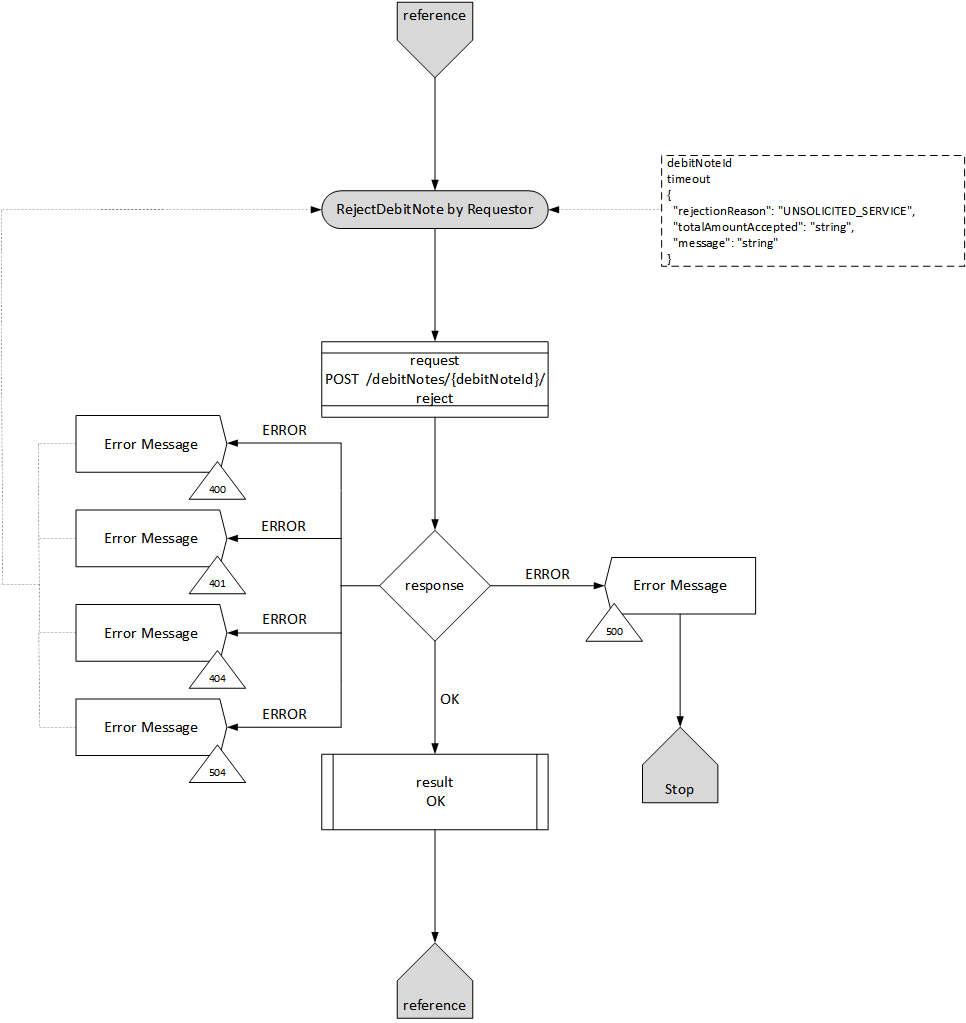
\includegraphics[width=12cm,height=12cm,angle=0]{./diag/Workflow/Payment/RejectDebitNote-R-Workflow.png}
    \caption{Requestor Workflow Accept Debit Note }
	\label{fig:RRDN}
\end{figure}


\end{enumerate}

\newpage

\subsubsubsubsection{IssueInvoice Function}

\begin{enumerate}

\item Profile

\begin{enumerate}

\item Description

The IssueInvoice function is used to create the Invoice Object by the Provider Node or Requestor Node. 
It uses the POST /invoices method.
The Invoice object indicates the total Amount owed by the Requestor in this Agreement. 
No further Debit Notes shall be issued after the Invoice is issued. 
The issue of Invoice signals the Termination of the Agreement (if it hasn't been terminated already). 
No Activity execution is allowed after the Invoice is issued.

\item Side

Both

\end{enumerate}

\item Request

\begin{enumerate}

\item Input

\begin{tcolorbox}[boxrule=0pt, frame empty]
\begin{verbatim}

No parameters

\end{verbatim}
\end{tcolorbox}

Object

\begin{tcolorbox}[boxrule=0pt, frame empty]
\begin{verbatim}

{
  "agreementId": "string",
  "activityIds": [
    "string"
  ],
  "amount": "string",
  "paymentDueDate": "YYYY-MM-DDThh:mm:ss.sssZ"
}

\end{verbatim}
\end{tcolorbox}

\begin{table}[H]
\footnotesize

\begin{center}
\begin{tabular}{|p{3cm}|l|p{3cm}|p{3cm}|p{4cm}|} 
\hline
\rowcolor{lightgray}	Name	& MO.	& Type	& Example & 	Description \\
\hline

activityIds				& M	& 	list(string)		&								&	List Activity Ids \\ 
\hline

amount					& M	& 	string				&								&	Amount  \\ 
\hline

agreementId				& M & 	string				&								&	Agreement Identifier \\
\hline

paymentDueDate			& M &	string(\$date-time)	&	YYYY-MM-DDThh:mm:ss.sssZ	&	Payment Due Date \\
\hline

\end{tabular}
\end{center}
\end{table}


\item REST Method

\begin{tcolorbox}[boxrule=0pt, frame empty]
\begin{verbatim} 

POST /invoices

\end{verbatim}
\end{tcolorbox}

\end{enumerate}

\item Response

\begin{table}[H]
\footnotesize

\begin{center}
\begin{tabular}{|c|l|} 
\hline
\rowcolor{lightgray}	Code 		& 	Description \\
\hline
201	 		&	OK \\
\hline
400			&	(400) Bad request \\
\hline
401			&	(401) Authorization information is missing or invalid. \\
\hline
500			&	(500) Server error. \\
\hline
\end{tabular}
\end{center}

\end{table}

\item Result

\begin{tcolorbox}[boxrule=0pt, frame empty]
\begin{verbatim}

{
  "invoiceId": "string",
  "issuerId": "string",
  "recipientId": "string",
  "payeeAddr": "string",
  "payerAddr": "string",
  "paymentPlatform": "string",
  "timestamp": "YYYY-MM-DDThh:mm:ss.sssZ",
  "agreementId": "string",
  "activityIds": [
    "string"
  ],
  "amount": "string",
  "paymentDueDate": "YYYY-MM-DDThh:mm:ss.sssZ",
  "status": "ISSUED"
}



\end{verbatim}
\end{tcolorbox}

\begin{table}[H]
\footnotesize

\begin{center}
\begin{tabular}{|p{3cm}|l|p{3cm}|p{3cm}|p{4cm}|} 
\hline
\rowcolor{lightgray}	Name	& MO.	& Type	& Example & 	Description \\
\hline

invoiceId				&	&	string				&																		&	Invoice Identifier \\
\hline   

issuerId				&	&	string				&																		&	Issuer Identifier \\
\hline   
  
recipientId				&	&	string				&																		&	Recipient Identifier \\
\hline   

payeeAddr				&	&	string				&																		&	Payee Address \\
\hline   
  
payerAddr				&	&	string				&																		&	Payer Address \\
\hline
   
paymentPlatform			&	&	object(string)		&																		&	Payment Platform Object \\
\hline

timestamp				&   &	string(\$date-time)	&	YYYY-MM-DDThh:mm:ss.sssZ											&	Time of ? \\
\hline

agreementId				& 	& 	string				&																		&	Agreement Identifier \\ 
\hline

activityIds				& 	& 	list(string)		&																		&	List Activity Ids \\ 
\hline

amount					& 	& 	string				&																		&	Amount  \\ 
\hline

paymentDueDate			&   &	string(\$date-time)	&	YYYY-MM-DDThh:mm:ss.sssZ											&	Payment Due Date \\
\hline

status					&	&	string(enum)		&	[ISSUED, RECEIVED, ACCEPTED, REJECTED, FAILED, SETTLED, CANCELLED]	& 	Debit Note state \\	
\hline

\end{tabular}
\end{center}
\end{table}

\item Workflow

(Please see Figure ~\ref{fig:PCI} on page ~\pageref{fig:PCI}):

\begin{figure}[htbp]
    \centering
    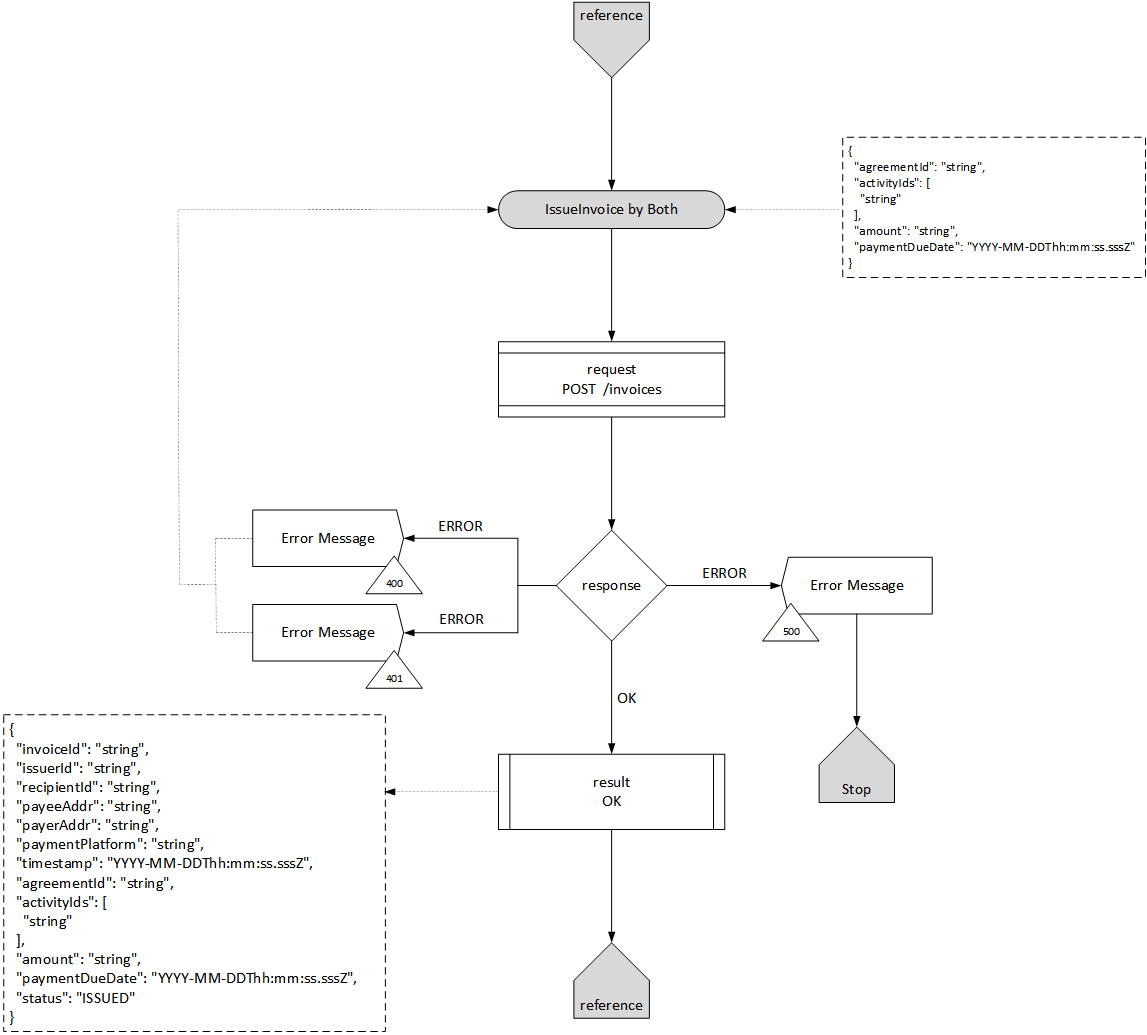
\includegraphics[width=12cm,height=12cm,angle=0]{./diag/Workflow/Payment/IssueInvoice-B-Workflow.png}
    \caption{Provider Workflow Create Invoice }
	\label{fig:PCI}
\end{figure}


\end{enumerate}

\newpage

%% List Invoices

\subsubsubsubsection{ListInvoices Function}

\begin{enumerate}

\item Profile

\begin{enumerate}

\item Description

The ListInvoices function is used to get the Invoice Objects by the Provider Node and Requestor Node. 
It uses the GET /invoices method.
 
\item Side

Both

\end{enumerate}

\item Request

\begin{enumerate}

\item Input

\begin{tcolorbox}[boxrule=0pt, frame empty]
\begin{verbatim}

afterTimestamp
maxItems

\end{verbatim}
\end{tcolorbox}

%Object
%\begin{tcolorbox}[boxrule=0pt, frame empty]
%\begin{verbatim}
%{
%  "activityId": "string",
%  "totalAmountDue": "string",
%  "usageCounterVector": {},
%  "paymentDueDate": "YYYY-MM-DDThh:mm:ss.sssZ"
%}
%\end{verbatim}
%\end{tcolorbox}

\begin{table}[H]
\footnotesize

\begin{center}
\begin{tabular}{|p{3cm}|l|p{3cm}|p{3cm}|p{4cm}|} 
\hline
\rowcolor{lightgray}	Name	& MO.	& Type	& Example & 	Description \\
\hline

maxItems				& O	& 	integer(\$int32)	&	10							&	Maximum number of items that server should return at once. \\ 
\hline

afterTimestamp			& O &	string(\$date-time)	&	YYYY-MM-DDThh:mm:ss.sssZ	&	Apply only to records created later than the specified timestamp \\
\hline

\end{tabular}
\end{center}
\end{table}


\item REST Method

\begin{tcolorbox}[boxrule=0pt, frame empty]
\begin{verbatim} 

GET /invoices

\end{verbatim}
\end{tcolorbox}

\end{enumerate}

\item Response

\begin{table}[H]
\footnotesize

\begin{center}
\begin{tabular}{|c|l|} 
\hline
\rowcolor{lightgray}	Code 		& 	Description \\
\hline
200	 		&	OK \\
\hline
401			&	(401) Authorization information is missing or invalid. \\
\hline
500			&	(500) Server error. \\
\hline
\end{tabular}
\end{center}

\end{table}

\item Result

\begin{tcolorbox}[boxrule=0pt, frame empty]
\begin{verbatim}

[
	{
		"invoiceId": "string",
		"issuerId": "string",
		"recipientId": "string",
		"payeeAddr": "string",
		"payerAddr": "string",
		"paymentPlatform": "string",
		"timestamp": "YYYY-MM-DDThh:mm:ss.sssZ",
		"agreementId": "string",
		"activityIds": [
			"string"
		],
		"amount": "string",
		"paymentDueDate": "YYYY-MM-DDThh:mm:ss.sssZ",
		"status": "ISSUED"
	}
]


\end{verbatim}
\end{tcolorbox}

\begin{table}[H]
\footnotesize

\begin{center}
\begin{tabular}{|p{3cm}|l|p{3cm}|p{3cm}|p{4cm}|} 
\hline
\rowcolor{lightgray}	Name	& MO.	& Type	& Example & 	Description \\
\hline

invoiceId				&	&	string				&																		&	Invoice Identifier \\
\hline   

issuerId				&	&	string				&																		&	Issuer Identifier \\
\hline   
  
recipientId				&	&	string				&																		&	Recipient Identifier \\
\hline   

payeeAddr				&	&	string				&																		&	Payee Address \\
\hline   
  
payerAddr				&	&	string				&																		&	Payer Address \\
\hline
   
paymentPlatform			&	&	object(string)		&																		&	Payment Platform Object \\
\hline

timestamp				&   &	string(\$date-time)	&	YYYY-MM-DDThh:mm:ss.sssZ											&	Time of ? \\
\hline

agreementId				& 	& 	string				&																		&	Agreement Identifier \\ 
\hline

activityIds				& 	& 	list(string)		&																		&	List Activity Ids \\ 
\hline

amount					& 	& 	string				&																		&	Amount  \\ 
\hline

paymentDueDate			&   &	string(\$date-time)	&	YYYY-MM-DDThh:mm:ss.sssZ											&	Payment Due Date \\
\hline

status					&	&	string(enum)		&	[ISSUED, RECEIVED, ACCEPTED, REJECTED, FAILED, SETTLED, CANCELLED]	& 	Debit Note state \\	
\hline

\end{tabular}
\end{center}
\end{table}

\item Workflow

(Please see Figure ~\ref{fig:BLI} on page ~\pageref{fig:BLI}):

\begin{figure}[htbp]
    \centering
    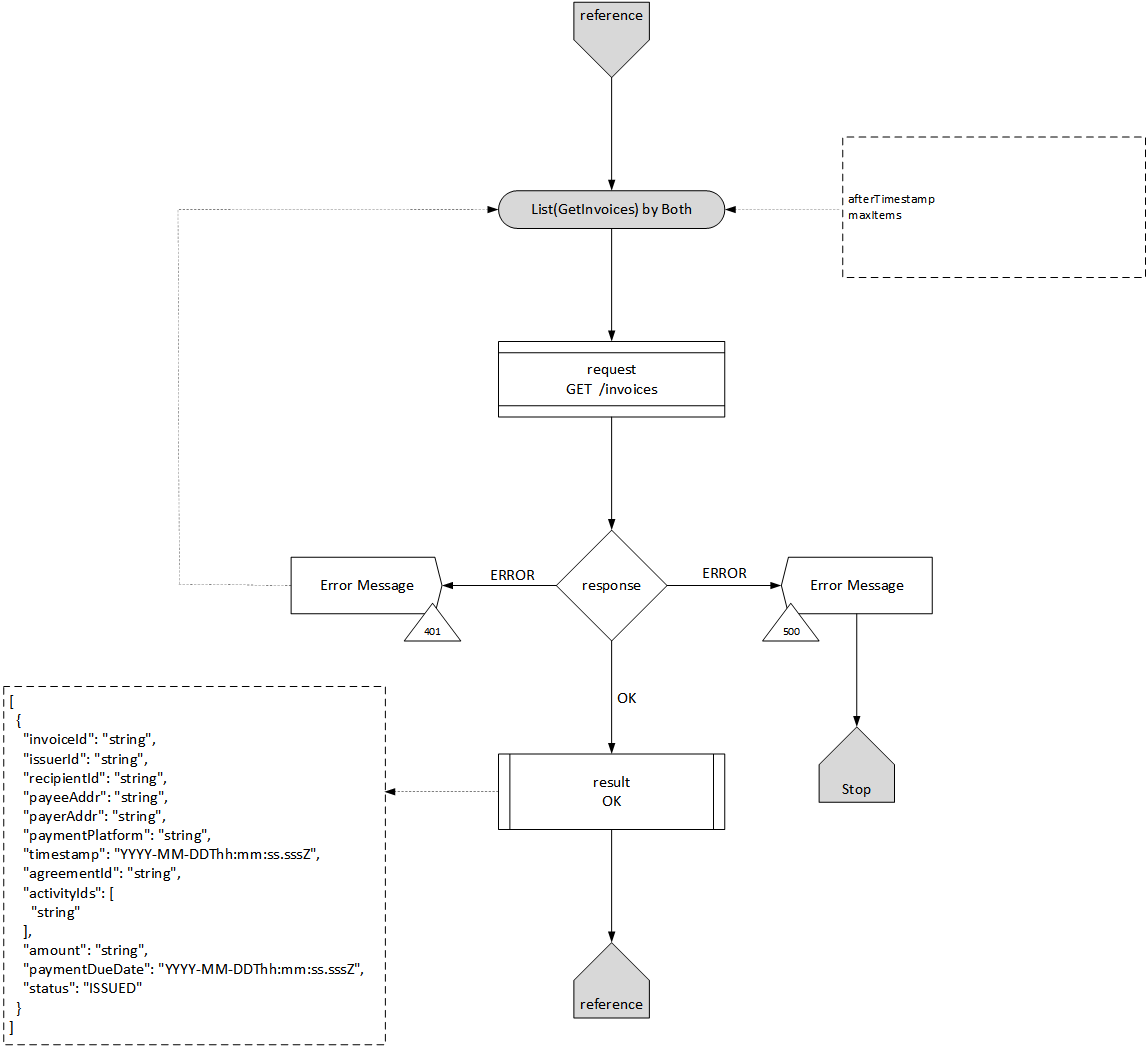
\includegraphics[width=12cm,height=12cm,angle=0]{./diag/Workflow/Payment/List(GetInvoices)-B-Workflow.png}
    \caption{Both Workflow List Invoices }
	\label{fig:BLI}
\end{figure}


\end{enumerate}

\newpage

%% Get Invoice

\subsubsubsubsection{GetInvoice Function}

\begin{enumerate}

\item Profile

\begin{enumerate}

\item Description

The GetInvoice function is used to get the Invoice Object by the Provider Node and Requestor Node. 
It uses the GET /invoices/\{invoiceId\} method.
 
\item Side

Both

\end{enumerate}

\item Request

\begin{enumerate}

\item Input

\begin{tcolorbox}[boxrule=0pt, frame empty]
\begin{verbatim}

invoiceId

\end{verbatim}
\end{tcolorbox}

%Object
%\begin{tcolorbox}[boxrule=0pt, frame empty]
%\begin{verbatim}
%{
%  "activityId": "string",
%  "totalAmountDue": "string",
%  "usageCounterVector": {},
%  "paymentDueDate": "YYYY-MM-DDThh:mm:ss.sssZ"
%}
%\end{verbatim}
%\end{tcolorbox}

\begin{table}[H]
\footnotesize

\begin{center}
\begin{tabular}{|p{3cm}|l|p{3cm}|p{3cm}|p{4cm}|} 
\hline
\rowcolor{lightgray}	Name	& MO.	& Type	& Example & 	Description \\
\hline

invoiceId				& M	& 	string				&								&	Invoice Identifier \\ 
\hline

%afterTimestamp			& O &	string(\$date-time)	&	YYYY-MM-DDThh:mm:ss.sssZ	&	Apply only to records created later than the specified timestamp \\
%\hline

\end{tabular}
\end{center}
\end{table}


\item REST Method

\begin{tcolorbox}[boxrule=0pt, frame empty]
\begin{verbatim} 

GET /invoices/{invoiceId}

\end{verbatim}
\end{tcolorbox}

\end{enumerate}

\item Response

\begin{table}[H]
\footnotesize

\begin{center}
\begin{tabular}{|c|l|} 
\hline
\rowcolor{lightgray}	Code 		& 	Description \\
\hline
200	 		&	OK \\
\hline
401			&	(401) Authorization information is missing or invalid. \\
\hline
404			&	(404) The specified resource was not found \\
\hline
500			&	(500) Server error. \\
\hline
\end{tabular}
\end{center}

\end{table}

\item Result

\begin{tcolorbox}[boxrule=0pt, frame empty]
\begin{verbatim}
	{
		"invoiceId": "string",
		"issuerId": "string",
		"recipientId": "string",
		"payeeAddr": "string",
		"payerAddr": "string",
		"paymentPlatform": "string",
		"timestamp": "YYYY-MM-DDThh:mm:ss.sssZ",
		"agreementId": "string",
		"activityIds": [
			"string"
		],
		"amount": "string",
		"paymentDueDate": "YYYY-MM-DDThh:mm:ss.sssZ",
		"status": "ISSUED"
	}
\end{verbatim}
\end{tcolorbox}

\begin{table}[H]
\footnotesize

\begin{center}
\begin{tabular}{|p{3cm}|l|p{3cm}|p{3cm}|p{4cm}|} 
\hline
\rowcolor{lightgray}	Name	& MO.	& Type	& Example & 	Description \\
\hline

invoiceId				&	&	string				&																		&	Invoice Identifier \\
\hline   

issuerId				&	&	string				&																		&	Issuer Identifier \\
\hline   
  
recipientId				&	&	string				&																		&	Recipient Identifier \\
\hline   

payeeAddr				&	&	string				&																		&	Payee Address \\
\hline   
  
payerAddr				&	&	string				&																		&	Payer Address \\
\hline
   
paymentPlatform			&	&	object(string)		&																		&	Payment Platform Object \\
\hline

timestamp				&   &	string(\$date-time)	&	YYYY-MM-DDThh:mm:ss.sssZ											&	Time of ? \\
\hline

agreementId				& 	& 	string				&																		&	Agreement Identifier \\ 
\hline

activityIds				& 	& 	list(string)		&																		&	List Activity Ids \\ 
\hline

amount					& 	& 	string				&																		&	Amount  \\ 
\hline

paymentDueDate			&   &	string(\$date-time)	&	YYYY-MM-DDThh:mm:ss.sssZ											&	Payment Due Date \\
\hline

status					&	&	string(enum)		&	[ISSUED, RECEIVED, ACCEPTED, REJECTED, FAILED, SETTLED, CANCELLED]	& 	Debit Note state \\	
\hline

\end{tabular}
\end{center}
\end{table}

\item Workflow

(Please see Figure ~\ref{fig:BGI} on page ~\pageref{fig:BGI}):

\begin{figure}[htbp]
    \centering
    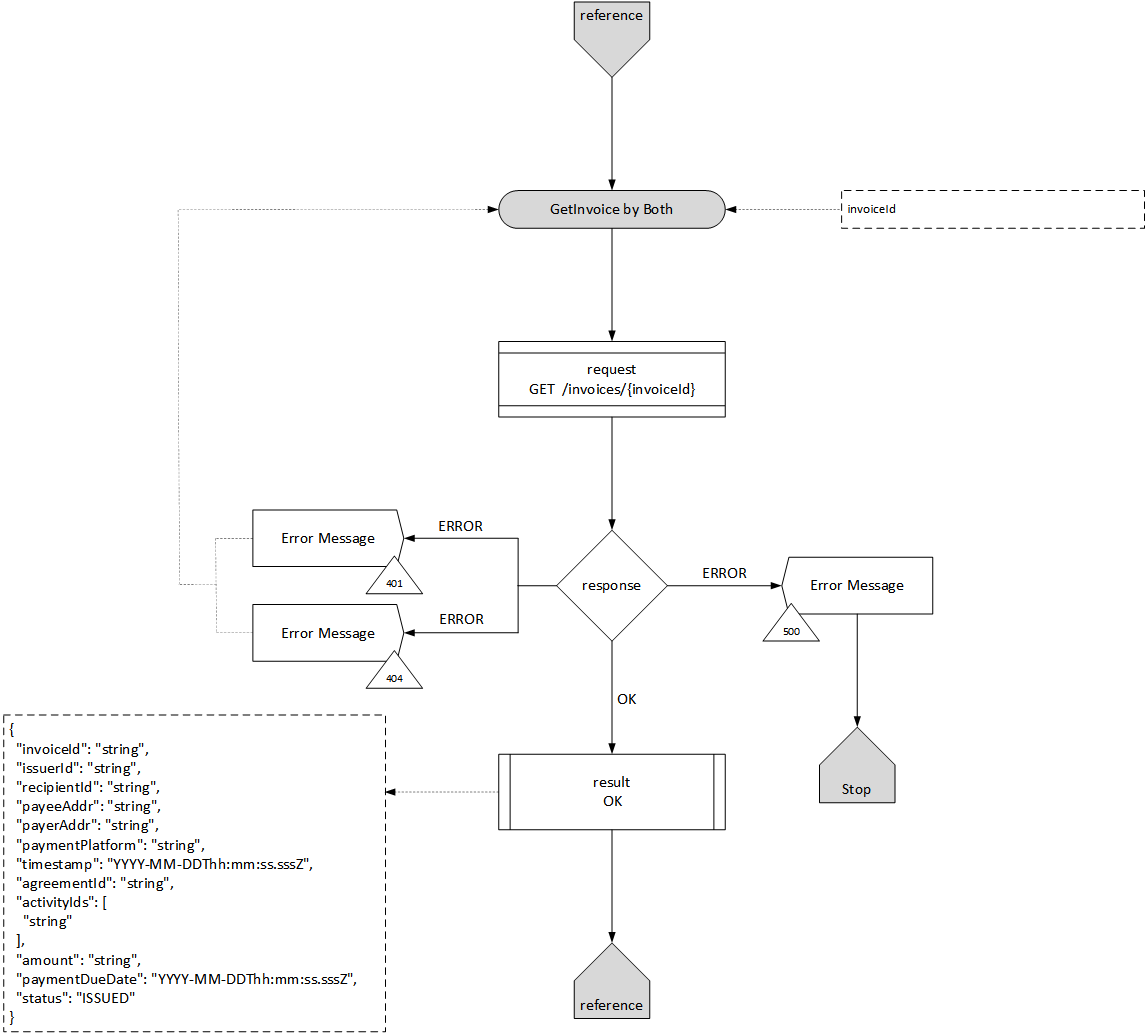
\includegraphics[width=12cm,height=12cm,angle=0]{./diag/Workflow/Payment/GetInvoice-B-Workflow.png}
    \caption{Both Workflow Get Invoice }
	\label{fig:BGI}
\end{figure}


\end{enumerate}

\newpage

%% InvoiceEvents

\subsubsubsubsection{CollectDebitNoteInvoiceEvent Function}

\begin{enumerate}

\item Profile

\begin{enumerate}

\item Description

The CollectDebitNoteInvoiceEvent function is used to get the Invoice events by the Provider Node and Requestor Node. 
It uses the GET /invoiceEvents method.
 
\item Side

Both

\end{enumerate}

\item Request

\begin{enumerate}

\item Input

\begin{tcolorbox}[boxrule=0pt, frame empty]
\begin{verbatim}

timeout
afterTimestamp
maxEvents
appSessionId

\end{verbatim}
\end{tcolorbox}

%Object
%\begin{tcolorbox}[boxrule=0pt, frame empty]
%\begin{verbatim}
%{
%  "activityId": "string",
%  "totalAmountDue": "string",
%  "usageCounterVector": {},
%  "paymentDueDate": "YYYY-MM-DDThh:mm:ss.sssZ"
%}
%\end{verbatim}
%\end{tcolorbox}

\begin{table}[H]
\footnotesize

\begin{center}
\begin{tabular}{|p{3cm}|l|p{3cm}|p{3cm}|p{4cm}|} 
\hline
\rowcolor{lightgray}	Name	& MO.	& Type	& Example & 	Description \\
\hline

timeout					& O	& 	number(\$float)		&	5							&	Timeout used in long-polling calls (in seconds). 
																						How many seconds server should wait for response containing new events 
																						(0.0 means it should return immediately if there are no events) \\ 
\hline

afterTimestamp			& O &	string(\$date-time)	&	YYYY-MM-DDThh:mm:ss.sssZ	&	Apply only to records created later than the specified timestamp \\
\hline

maxEvents				& O & 	integer(\$int32)	&	10							&	Maximum number of events that server should return at once. \\
\hline

appSessionId			& O &	string				&								&	A correlation/session identifier used for querying events related to 
																						an action where this appSessionId has been specified \\
\hline

\end{tabular}
\end{center}
\end{table}


\item REST Method

\begin{tcolorbox}[boxrule=0pt, frame empty]
\begin{verbatim} 

GET /invoiceEvents

\end{verbatim}
\end{tcolorbox}

\end{enumerate}

\item Response

\begin{table}[H]
\footnotesize

\begin{center}
\begin{tabular}{|c|l|} 
\hline
\rowcolor{lightgray}	Code 		& 	Description \\
\hline
200	 		&	OK \\
\hline
401			&	(401) Authorization information is missing or invalid. \\
\hline
%404		&	(404) The specified resource was not found \\
%\hline
500			&	(500) Server error. \\
\hline
\end{tabular}
\end{center}

\end{table}

\item Result

\begin{tcolorbox}[boxrule=0pt, frame empty]
\begin{verbatim}

[
  {
    "eventType": "string",
    "eventDate": "YYYY-MM-DDThh:mm:ss.sssZ",
    "invoiceId": "string"
  }
]


\end{verbatim}
\end{tcolorbox}

\begin{table}[H]
\footnotesize

\begin{center}
\begin{tabular}{|p{3cm}|l|p{3cm}|p{3cm}|p{4cm}|} 
\hline
\rowcolor{lightgray}	Name	& MO.	& Type	& Example & 	Description \\
\hline

invoiceId				&	&	string				&																		&	Invoice Identifier \\
\hline   

eventDate				&   &	string(\$date-time)	&	YYYY-MM-DDThh:mm:ss.sssZ											&	Event Date \\
\hline

eventType				&	&	string				&																		& 	Event Type \\	
\hline

\end{tabular}
\end{center}
\end{table}

\item Workflow

(Please see Figure ~\ref{fig:BGIE} on page ~\pageref{fig:BGIE}):

\begin{figure}[htbp]
    \centering
    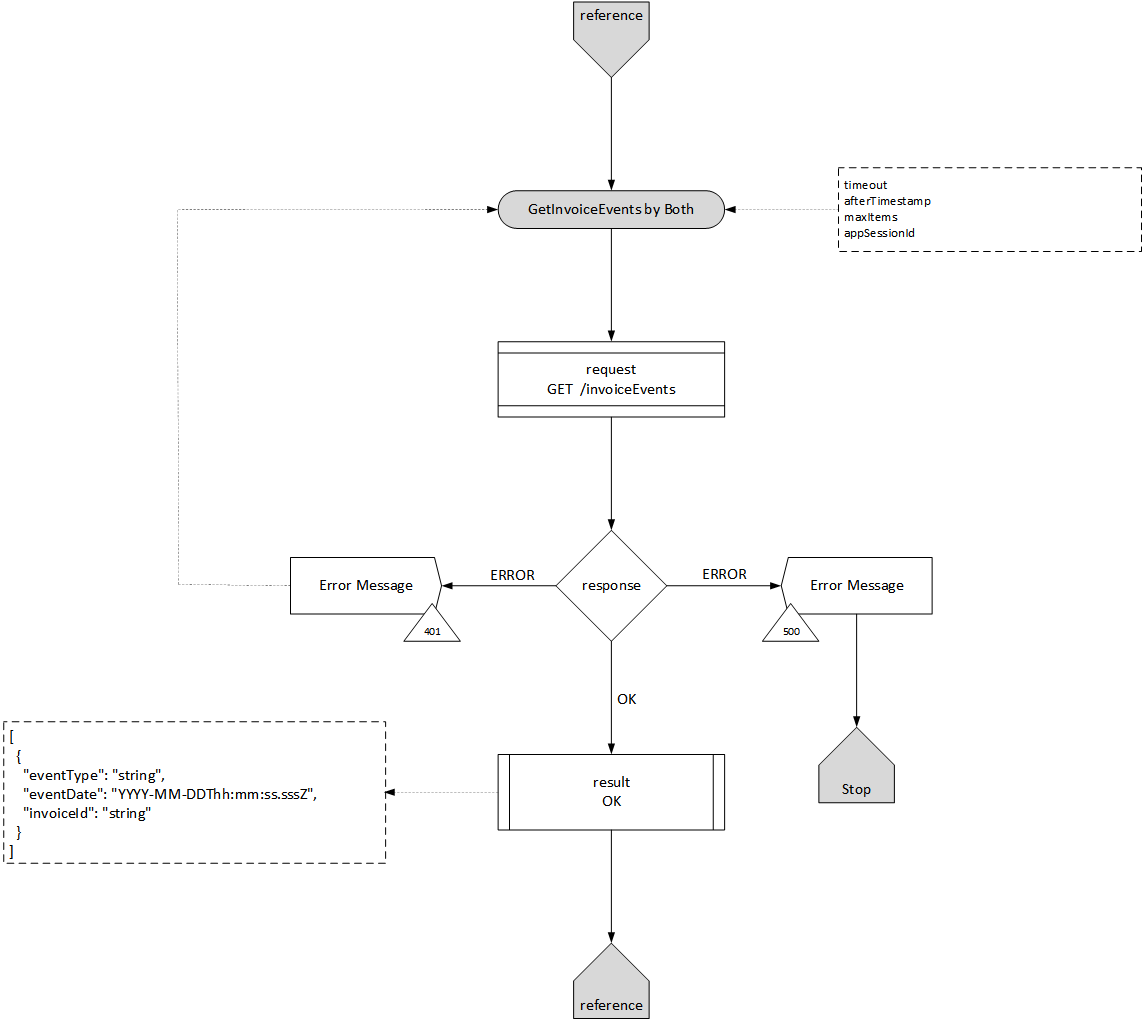
\includegraphics[width=12cm,height=12cm,angle=0]{./diag/Workflow/Payment/InvoiceEvents-B-Workflow.png}
    \caption{Both Workflow Get Invoice Events }
	\label{fig:BGIE}
\end{figure}


\end{enumerate}

\newpage

% SendInvoice 

\subsubsubsubsection{SendInvoice Function}

\begin{enumerate}

\item Profile

\begin{enumerate}

\item Description

The SendInvoice function is used to send the Invoice Object from the Provider Node to the Requestor Node. 
It uses the POST /invoices/\{invoiceId\}/send method.

\item Side

Provider

\end{enumerate}

\item Request

\begin{enumerate}

\item Input

\begin{tcolorbox}[boxrule=0pt, frame empty]
\begin{verbatim}

invoiceId
timeout

\end{verbatim}
\end{tcolorbox}

%Object

%\begin{tcolorbox}[boxrule=0pt, frame empty]
%\begin{verbatim}

%{
%  "activityId": "string",
%  "totalAmountDue": "string",
%  "usageCounterVector": {},
%  "paymentDueDate": "YYYY-MM-DDThh:mm:ss.sssZ"
%}

%\end{verbatim}
%\end{tcolorbox}

\begin{table}[H]
\footnotesize

\begin{center}
\begin{tabular}{|p{3cm}|l|p{3cm}|p{3cm}|p{4cm}|} 
\hline
\rowcolor{lightgray}	Name	& MO.	& Type	& Example & 	Description \\
\hline

invoiceId				& M	&	string				&								&	Invoice Identifier \\
\hline   

timeout					& O &	number(\$float)		&	5							&	Timeout used in blocking calls waiting for eg. acknowledgement. 
																						How many seconds server should wait for response/acknowledgement 
																						of an action 
																						(0.0 means it should wait for other party's response indefinitely) \\
\hline

\end{tabular}
\end{center}
\end{table}


\item REST Method

\begin{tcolorbox}[boxrule=0pt, frame empty]
\begin{verbatim} 

POST /invoices/{invoiceId}/send

\end{verbatim}
\end{tcolorbox}

\end{enumerate}

\item Response

\begin{table}[H]
\footnotesize

\begin{center}
\begin{tabular}{|c|l|} 
\hline
\rowcolor{lightgray}	Code 		& 	Description \\
\hline
200	 		&	OK \\
\hline
404			&	(404) The specified resource was not found. \\
\hline
401			&	(401) Authorization information is missing or invalid. \\
\hline
500			&	(500) Server error. \\
\hline
504			&	(504) Ack timeout. \\
\hline

\end{tabular}
\end{center}

\end{table}

\item Result

\begin{tcolorbox}[boxrule=0pt, frame empty]
\begin{verbatim}

As above

\end{verbatim}
\end{tcolorbox}

%\begin{table}
%\footnotesize
%\begin{center}
%\begin{tabular}{|p{3cm}|l|p{3cm}|p{3cm}|p{4cm}|} 
%\hline
%\rowcolor{lightgray}	Name	& MO.	& Type	& Example & 	Description \\
%\hline	
%\end{tabular}
%\end{center}
%\end{table}

\item Workflow

(Please see Figure ~\ref{fig:PSI} on page ~\pageref{fig:PSI}):

\begin{figure}[htbp]
    \centering
    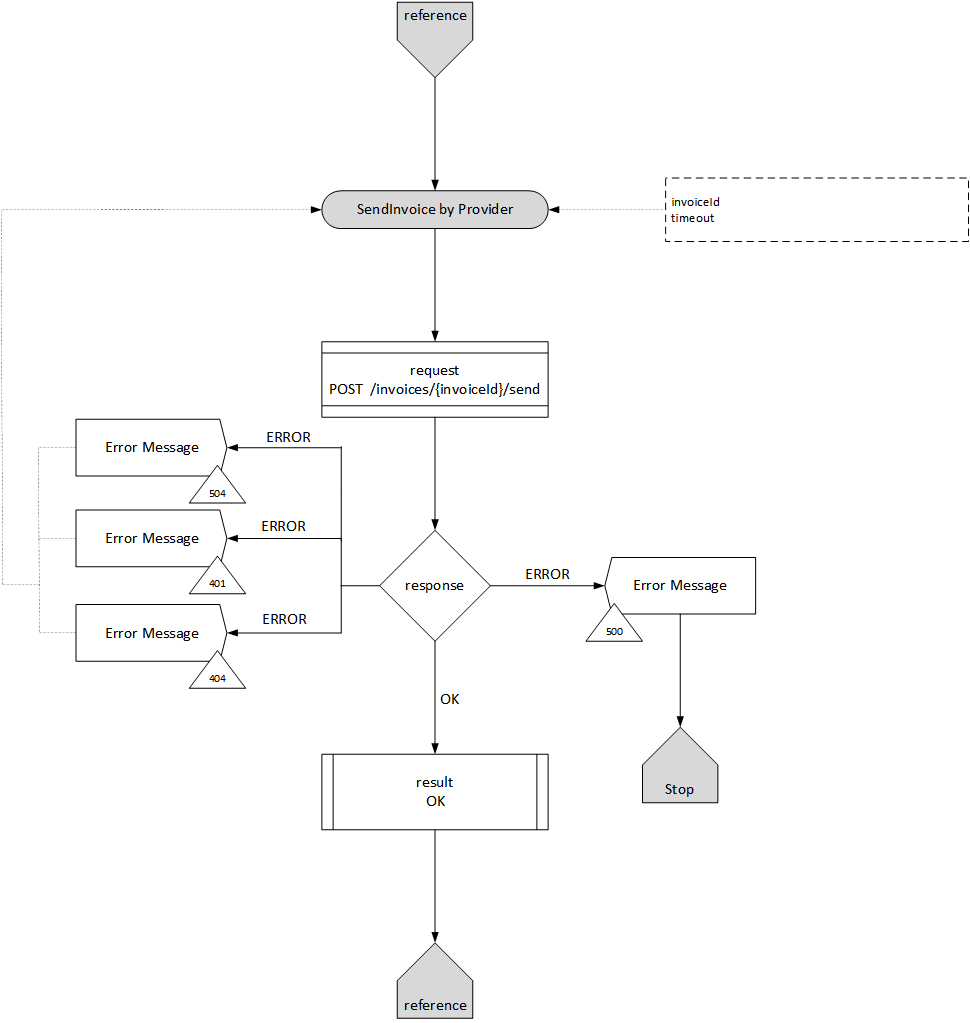
\includegraphics[width=12cm,height=12cm,angle=0]{./diag/Workflow/Payment/SendInvoice-P-Workflow.png}
    \caption{Provider Workflow Send Invoice }
	\label{fig:PSI}
\end{figure}


\end{enumerate}

\newpage


% AcceptInvoice 

\subsubsubsubsection{AcceptInvoice Function}

\begin{enumerate}

\item Profile

\begin{enumerate}

\item Description

The AcceptInvoice function is used to accept received the Invoice Object by the Requestor Node. 
It uses the POST /invoices/\{invoiceId\}/accept method.

\item Side

Requestor

\end{enumerate}

\item Request

\begin{enumerate}

\item Input

\begin{tcolorbox}[boxrule=0pt, frame empty]
\begin{verbatim}

invoiceId
timeout

\end{verbatim}
\end{tcolorbox}

Object

\begin{tcolorbox}[boxrule=0pt, frame empty]
\begin{verbatim}

{
  "totalAmountAccepted": "string",
  "allocationId": "string",
}

\end{verbatim}
\end{tcolorbox}

\begin{table}[H]
\footnotesize

\begin{center}
\begin{tabular}{|p{3cm}|l|p{3cm}|p{3cm}|p{4cm}|} 
\hline
\rowcolor{lightgray}	Name	& MO.	& Type	& Example & 	Description \\
\hline

invoiceId				& M	&	string				&								&	Invoice Identifier \\
\hline   

timeout					& O &	number(\$float)		&	5							&	Timeout used in blocking calls waiting for eg. acknowledgement. 
																						How many seconds server should wait for response/acknowledgement 
																						of an action 
																						(0.0 means it should wait for other party's response indefinitely) \\
\hline

totalAmountAccepted		& M &	string				&								&			\\
\hline

allocationId			& M &  	string				&								&			\\
\hline

\end{tabular}
\end{center}
\end{table}


\item REST Method

\begin{tcolorbox}[boxrule=0pt, frame empty]
\begin{verbatim} 

POST /invoices/{invoiceId}/accept

\end{verbatim}
\end{tcolorbox}

\end{enumerate}

\item Response

\begin{table}[H]
\footnotesize

\begin{center}
\begin{tabular}{|c|l|} 
\hline
\rowcolor{lightgray}	Code 		& 	Description \\
\hline
200	 		&	OK \\
\hline
400			&	(400) Bad request \\
\hline
404			&	(404) The specified resource was not found. \\
\hline
401			&	(401) Authorization information is missing or invalid. \\
\hline
500			&	(500) Server error. \\
\hline
504			&	(504) Ack timeout. \\
\hline

\end{tabular}
\end{center}

\end{table}

\item Result

\begin{tcolorbox}[boxrule=0pt, frame empty]
\begin{verbatim}

As above

\end{verbatim}
\end{tcolorbox}

%\begin{table}
%\footnotesize
%\begin{center}
%\begin{tabular}{|p{3cm}|l|p{3cm}|p{3cm}|p{4cm}|} 
%\hline
%\rowcolor{lightgray}	Name	& MO.	& Type	& Example & 	Description \\
%\hline	
%\end{tabular}
%\end{center}
%\end{table}

\item Workflow

(Please see Figure ~\ref{fig:RAI} on page ~\pageref{fig:RAI}):

\begin{figure}[htbp]
    \centering
    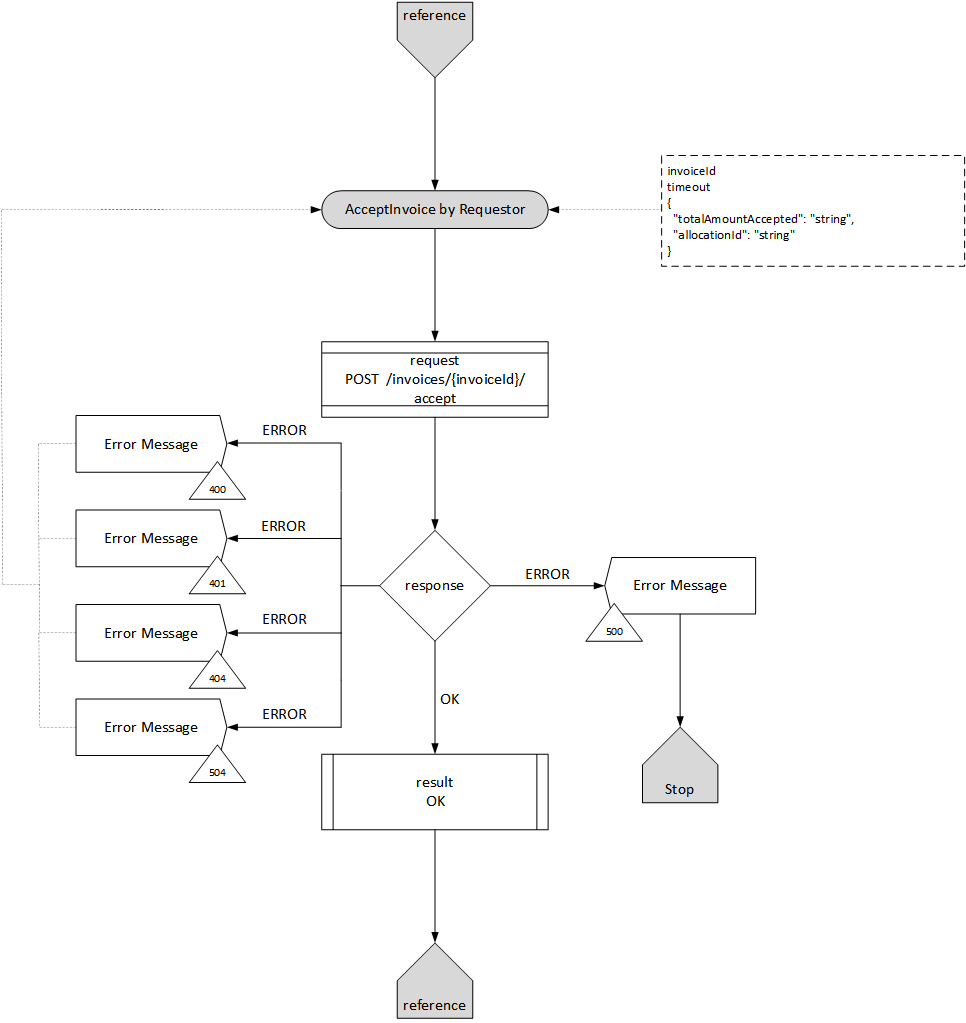
\includegraphics[width=12cm,height=12cm,angle=0]{./diag/Workflow/Payment/AcceptInvoice-R-Workflow.png}
    \caption{Requestor Workflow Accept Invoice }
	\label{fig:RAI}
\end{figure}


\end{enumerate}

\newpage

% RejectInvoice  %%%

\subsubsubsubsection{RejectInvoice Function}

\begin{enumerate}

\item Profile

\begin{enumerate}

\item Description

The RejectInvoice function is used to reject received the Invoice Object by the Requestor Node. 
It uses the POST /invoices/\{invoiceId\}/reject method.

\item Side

Requestor

\end{enumerate}

\item Request

\begin{enumerate}

\item Input

\begin{tcolorbox}[boxrule=0pt, frame empty]
\begin{verbatim}

invoiceId
timeout

\end{verbatim}
\end{tcolorbox}

Object

\begin{tcolorbox}[boxrule=0pt, frame empty]
\begin{verbatim}

{
  "rejectionReason": "UNSOLICITED_SERVICE",
  "totalAmountAccepted": "string",
  "message": "string"
}

\end{verbatim}
\end{tcolorbox}

\begin{table}[H]
\footnotesize

\begin{center}
\begin{tabular}{|p{3cm}|l|p{3cm}|p{3cm}|p{4cm}|} 
\hline
\rowcolor{lightgray}	Name	& MO.	& Type	& Example & 	Description \\
\hline

invoiceId				& M	&	string				&								&	Invoice Identifier \\
\hline   

timeout					& O &	number(\$float)		&	5							&	Timeout used in blocking calls waiting for eg. acknowledgement. 
																						How many seconds server should wait for response/acknowledgement 
																						of an action 
																						(0.0 means it should wait for other party's response indefinitely) \\
\hline

totalAmountAccepted		& M &	string				&								&			\\
\hline

message					& M &  	string				&								&			\\
\hline

rejectionReason 		& M & 	string(enum)		&	[UNSOLICITED\_SERVICE, BAD\_SERVICE, INCORRECT\_AMOUNT]	&	Possible reasons to reject a Debit Note		\\
\hline

\end{tabular}
\end{center}
\end{table}


\item REST Method

\begin{tcolorbox}[boxrule=0pt, frame empty]
\begin{verbatim} 

POST /invoices/{invoiceId}/reject

\end{verbatim}
\end{tcolorbox}

\end{enumerate}

\item Response

\begin{table}[H]
\footnotesize

\begin{center}
\begin{tabular}{|c|l|} 
\hline
\rowcolor{lightgray}	Code 		& 	Description \\
\hline
200	 		&	OK \\
\hline
400			&	(400) Bad request \\
\hline
404			&	(404) The specified resource was not found. \\
\hline
401			&	(401) Authorization information is missing or invalid. \\
\hline
500			&	(500) Server error. \\
\hline
504			&	(504) Ack timeout. \\
\hline

\end{tabular}
\end{center}

\end{table}

\item Result

\begin{tcolorbox}[boxrule=0pt, frame empty]
\begin{verbatim}

As above

\end{verbatim}
\end{tcolorbox}

%\begin{table}
%\footnotesize
%\begin{center}
%\begin{tabular}{|p{3cm}|l|p{3cm}|p{3cm}|p{4cm}|} 
%\hline
%\rowcolor{lightgray}	Name	& MO.	& Type	& Example & 	Description \\
%\hline	
%\end{tabular}
%\end{center}
%\end{table}

\item Workflow

(Please see Figure ~\ref{fig:RRI} on page ~\pageref{fig:RRI}):

\begin{figure}[htbp]
    \centering
    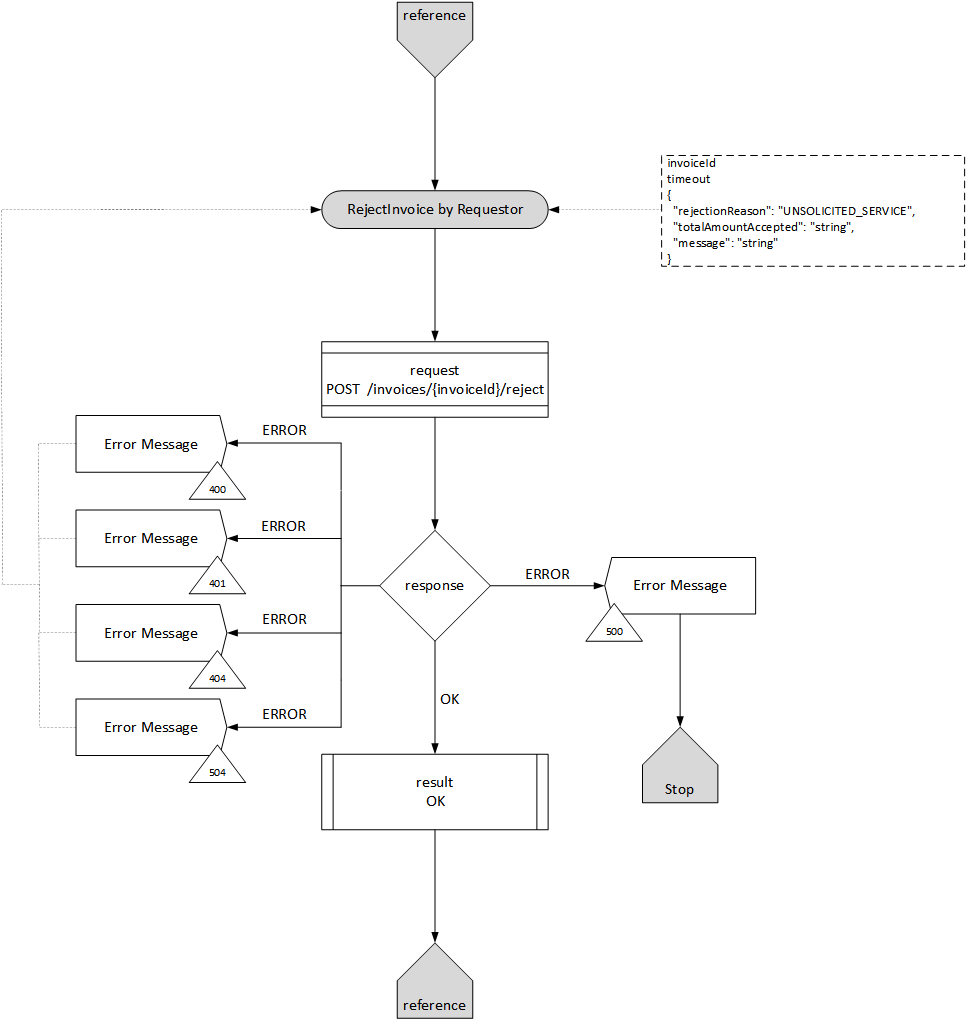
\includegraphics[width=12cm,height=12cm,angle=0]{./diag/Workflow/Payment/RejectInvoice-R-Workflow.png}
    \caption{Requestor Workflow Accept Invoice }
	\label{fig:RRI}
\end{figure}


\end{enumerate}

\newpage

%% Get Allocation

\subsubsubsubsection{GetAllocation Function}

\begin{enumerate}

\item Profile

\begin{enumerate}

\item Description

The GetAllocation function is used to get the Allocation Object by Requestor Node. 
It uses the GET /allocations/\{allocationId\} method.

An Allocation is a designated sum of money reserved for the purpose of making some particular payments. 
Allocations are currently purely virtual objects. They only exist in the Requestor node database.
An Allocation is connected to a payment account (wallet) specified by address and paymentPlatform field. 
If these fields are not present the default payment platform is used and the address is assumed 
to be identical to the Requestor's Node ID.

 
\item Side

Requestor

\end{enumerate}

\item Request

\begin{enumerate}

\item Input

\begin{tcolorbox}[boxrule=0pt, frame empty]
\begin{verbatim}

allocationId

\end{verbatim}
\end{tcolorbox}

%Object
%\begin{tcolorbox}[boxrule=0pt, frame empty]
%\begin{verbatim}
%{
%  "activityId": "string",
%  "totalAmountDue": "string",
%  "usageCounterVector": {},
%  "paymentDueDate": "YYYY-MM-DDThh:mm:ss.sssZ"
%}
%\end{verbatim}
%\end{tcolorbox}

\begin{table}[H]
\footnotesize

\begin{center}
\begin{tabular}{|p{3cm}|l|p{3cm}|p{3cm}|p{4cm}|} 
\hline
\rowcolor{lightgray}	Name	& MO.	& Type	& Example & 	Description \\
\hline

allocationId				& M	& 	string				&								&	Allocation Identifier \\ 
\hline

%afterTimestamp				& O &	string(\$date-time)	&	YYYY-MM-DDThh:mm:ss.sssZ	&	Apply only to records created later than the specified timestamp \\
%\hline

\end{tabular}
\end{center}
\end{table}


\item REST Method

\begin{tcolorbox}[boxrule=0pt, frame empty]
\begin{verbatim} 

GET /allocations/{allocationId}

\end{verbatim}
\end{tcolorbox}

\end{enumerate}

\item Response

\begin{table}[H]
\footnotesize

\begin{center}
\begin{tabular}{|c|l|} 
\hline
\rowcolor{lightgray}	Code 		& 	Description \\
\hline
200	 		&	OK \\
\hline
401			&	(401) Authorization information is missing or invalid. \\
\hline
404			&	(404) The specified resource was not found \\
\hline
500			&	(500) Server error. \\
\hline
\end{tabular}
\end{center}

\end{table}

\item Result

\begin{tcolorbox}[boxrule=0pt, frame empty]
\begin{verbatim}

{
  "allocationId": "string",
  "address": "string",
  "paymentPlatform": {
    "driver": "string",
    "network": "string",
    "token": "string"
  },
  "totalAmount": "string",
  "spentAmount": "string",
  "remainingAmount": "string",
  "timestamp": "YYYY-MM-DDThh:mm:ss.sssZ",
  "timeout": "YYYY-MM-DDThh:mm:ss.sssZ",
  "makeDeposit": true,
  "extendTimeout": 0,
  "deposit": {
    "id": "string",
    "contract": "string",
    "validate": {}
  }
}



\end{verbatim}
\end{tcolorbox}

\begin{table}[H]
\footnotesize

\begin{center}
\begin{tabular}{|p{3cm}|l|p{3cm}|p{3cm}|p{4cm}|} 
\hline
\rowcolor{lightgray}	Name	& MO.	& Type	& Example & 	Description \\
\hline

allocationId				&	&	string				&								&	Allocation Identifier \\
\hline   

address						&	&	string				&								&	Address	 \\
\hline   
  
paymentPlatform. driver		&	&	string				&								&	Payment Platform Driver \\
\hline   

paymentPlatform. network	&	&	string				&								&	Payment Platform Network \\
\hline   
  
paymentPlatform. token		&	&	string				&								&	Payment Platform Token \\
\hline
     
totalAmount					&	&	string				&								&	Total Amount \\
\hline

spentAmount					&	&	string				&								&	Spent Amount \\
\hline

remainingAmount				&	&	string				&								&	Remaining Amount \\
\hline

timestamp					&   &	string(\$date-time)	&	YYYY-MM-DDThh:mm:ss.sssZ	&	Time of ? \\
\hline

timeout						& 	& 	string(\$date-time)	&	YYYY-MM-DDThh:mm:ss.sssZ	&	Timeout \\ 
\hline

makeDeposit					& 	& 	boolean				&	[true, false]				&	Make Deposit \\ 
\hline

extendTimeout				& 	& 	integer(\$int64)	&	0							&	Extend Timeout \\ 
\hline

deposit.id					&   & 	string				&								&	Deposit Identifier \\
\hline

deposit.contract			&   &	string				&								&	Deposit Contract \\
\hline

deposit.validate			&   &	json				&								&	Deposit Validate \\
\hline

\end{tabular}
\end{center}
\end{table}

\item Workflow

(Please see Figure ~\ref{fig:RGA} on page ~\pageref{fig:RGA}):

\begin{figure}[htbp]
    \centering
    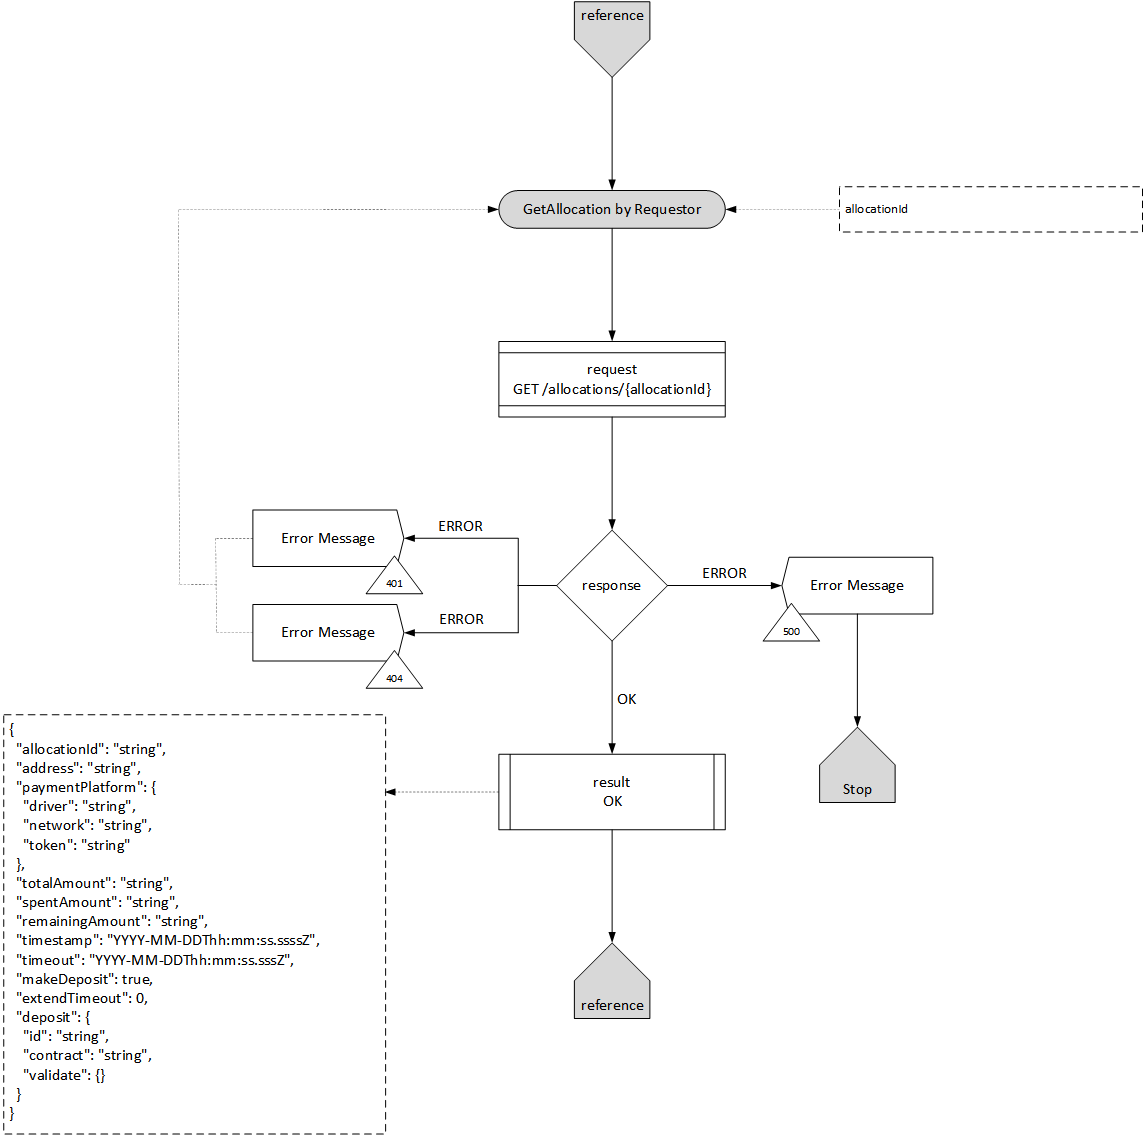
\includegraphics[width=12cm,height=12cm,angle=0]{./diag/Workflow/Payment/GetAllocation-R-Workflow.png}
    \caption{Requestor Workflow Get Allocation }
	\label{fig:RGA}
\end{figure}


\end{enumerate}

\newpage

%% List Allocations

\subsubsubsubsection{ListAllocations Function}

\begin{enumerate}

\item Profile

\begin{enumerate}

\item Description

The ListAllocations function is used to get the Allocation Objects by Requestor Node. 
It uses the GET /allocations method.

An Allocation is a designated sum of money reserved for the purpose of making some particular payments. 
Allocations are currently purely virtual objects. They only exist in the Requestor node database.
An Allocation is connected to a payment account (wallet) specified by address and paymentPlatform field. 
If these fields are not present the default payment platform is used and the address is assumed 
to be identical to the Requestor's Node ID.

 
\item Side

Requestor

\end{enumerate}

\item Request

\begin{enumerate}

\item Input

\begin{tcolorbox}[boxrule=0pt, frame empty]
\begin{verbatim}

No parameters

\end{verbatim}
\end{tcolorbox}

%Object
%\begin{tcolorbox}[boxrule=0pt, frame empty]
%\begin{verbatim}
%{
%  "activityId": "string",
%  "totalAmountDue": "string",
%  "usageCounterVector": {},
%  "paymentDueDate": "YYYY-MM-DDThh:mm:ss.sssZ"
%}
%\end{verbatim}
%\end{tcolorbox}

%\begin{table}[H]
%\footnotesize

%\begin{center}
%\begin{tabular}{|p{3cm}|l|p{3cm}|p{3cm}|p{4cm}|} 
%\hline
%\rowcolor{lightgray}	Name	& MO.	& Type	& Example & 	Description \\
%\hline
%allocationId		& M	& 	string				&								&	Allocation Identifier \\ 
%\hline
%afterTimestamp		& O &	string(\$date-time)	&	YYYY-MM-DDThh:mm:ss.sssZ	&	Apply only to records created later than the specified timestamp \\
%\hline
%\end{tabular}
%\end{center}
%\end{table}

\item REST Method

\begin{tcolorbox}[boxrule=0pt, frame empty]
\begin{verbatim} 

GET /allocations

\end{verbatim}
\end{tcolorbox}

\end{enumerate}

\item Response

\begin{table}[H]
\footnotesize

\begin{center}
\begin{tabular}{|c|l|} 
\hline
\rowcolor{lightgray}	Code 		& 	Description \\
\hline
200	 		&	OK \\
\hline
401			&	(401) Authorization information is missing or invalid. \\
\hline
500			&	(500) Server error. \\
\hline
\end{tabular}
\end{center}

\end{table}

\item Result

\begin{tcolorbox}[boxrule=0pt, frame empty]
\begin{verbatim}

[
 {
  "allocationId": "string",
  "address": "string",
  "paymentPlatform": {
    "driver": "string",
    "network": "string",
    "token": "string"
  },
  "totalAmount": "string",
  "spentAmount": "string",
  "remainingAmount": "string",
  "timestamp": "YYYY-MM-DDThh:mm:ss.sssZ",
  "timeout": "YYYY-MM-DDThh:mm:ss.sssZ",
  "makeDeposit": true,
  "extendTimeout": 0,
  "deposit": {
    "id": "string",
    "contract": "string",
    "validate": {}
  }
 }
]

\end{verbatim}
\end{tcolorbox}

\begin{table}[H]
\footnotesize

\begin{center}
\begin{tabular}{|p{3cm}|l|p{3cm}|p{3cm}|p{4cm}|} 
\hline
\rowcolor{lightgray}	Name	& MO.	& Type	& Example & 	Description \\
\hline

allocationId				&	&	string				&								&	Allocation Identifier \\
\hline   

address						&	&	string				&								&	Address	 \\
\hline   
  
paymentPlatform. driver		&	&	string				&								&	Payment Platform Driver \\
\hline   

paymentPlatform. network	&	&	string				&								&	Payment Platform Network \\
\hline   
  
paymentPlatform. token		&	&	string				&								&	Payment Platform Token \\
\hline
     
totalAmount					&	&	string				&								&	Total Amount \\
\hline

spentAmount					&	&	string				&								&	Spent Amount \\
\hline

remainingAmount				&	&	string				&								&	Remaining Amount \\
\hline

timestamp					&   &	string(\$date-time)	&	YYYY-MM-DDThh:mm:ss.sssZ	&	Time of ? \\
\hline

timeout						& 	& 	string(\$date-time)	&	YYYY-MM-DDThh:mm:ss.sssZ	&	Timeout \\ 
\hline

makeDeposit					& 	& 	boolean				&	[true, false]				&	Make Deposit \\ 
\hline

extendTimeout				& 	& 	integer(\$int64)	&	0							&	Extend Timeout \\ 
\hline

deposit.id					&   & 	string				&								&	Deposit Identifier \\
\hline

deposit.contract			&   &	string				&								&	Deposit Contract \\
\hline

deposit.validate			&   &	json				&								&	Deposit Validate \\
\hline

\end{tabular}
\end{center}
\end{table}

\item Workflow

(Please see Figure ~\ref{fig:RLA} on page ~\pageref{fig:RLA}):

\begin{figure}[htbp]
    \centering
    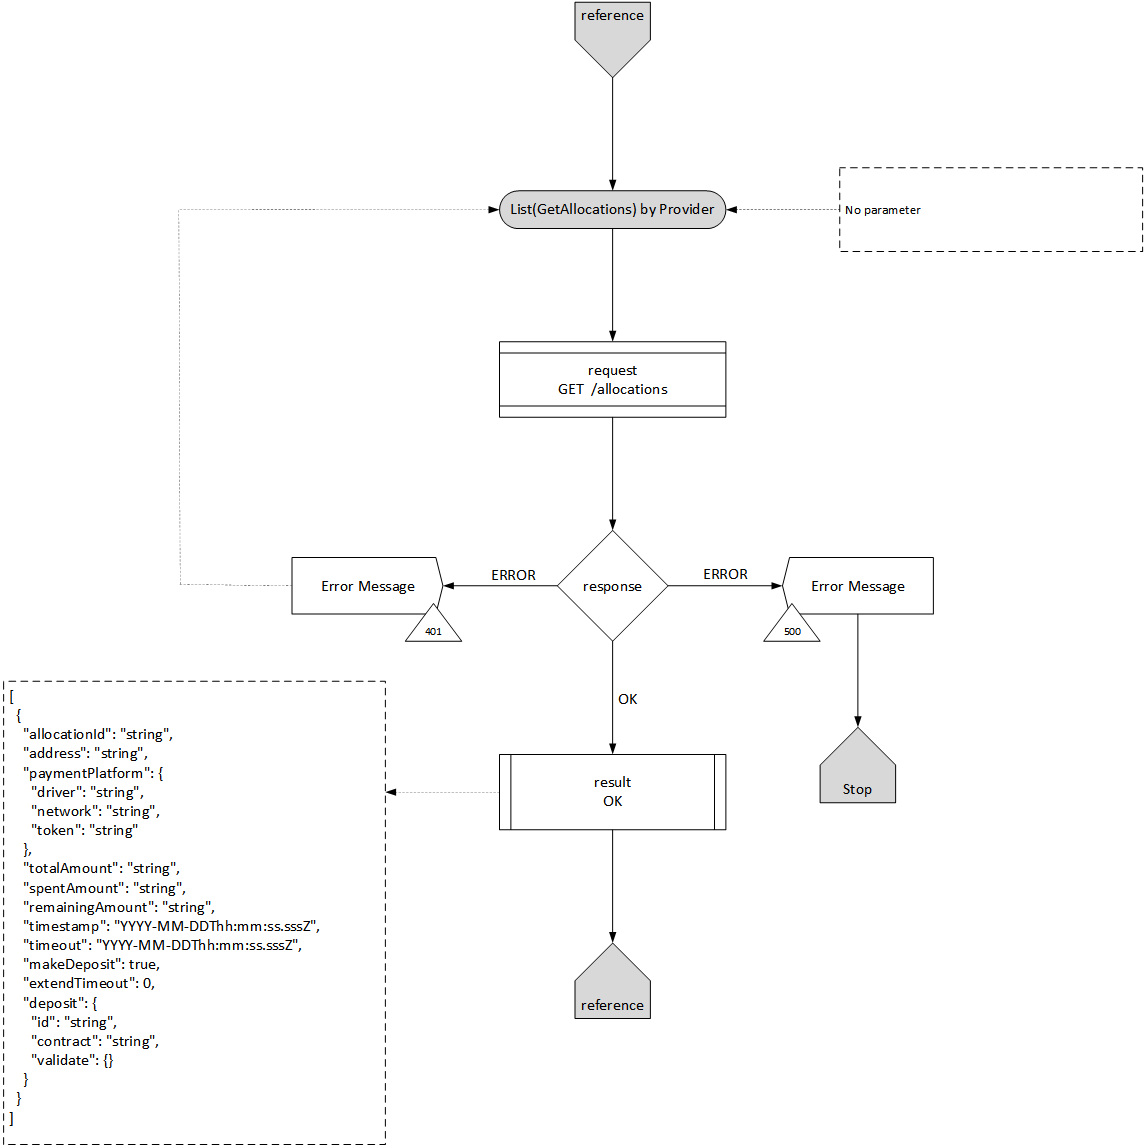
\includegraphics[width=12cm,height=12cm,angle=0]{./diag/Workflow/Payment/List(GetAllocations)-R-Workflow.png}
    \caption{Requestor Workflow List Allocations }
	\label{fig:RLA}
\end{figure}


\end{enumerate}

\newpage

%% AllocateAmount

\subsubsubsubsection{AllocateAmount Function}

\begin{enumerate}

\item Profile

\begin{enumerate}

\item Description

The AllocateAmount function is used to create the Allocation Objects by Requestor Node. 
It uses the POST /allocations method.

An Allocation is a designated sum of money reserved for the purpose of making some particular payments. 
Allocations are currently purely virtual objects. They only exist in the Requestor node database.
An Allocation is connected to a payment account (wallet) specified by address and paymentPlatform field. 
If these fields are not present the default payment platform is used and the address is assumed 
to be identical to the Requestor's Node ID.

 
\item Side

Requestor

\end{enumerate}

\item Request

\begin{enumerate}

\item Input

\begin{tcolorbox}[boxrule=0pt, frame empty]
\begin{verbatim}

afterTimestamp
maxItems

\end{verbatim}
\end{tcolorbox}

Object
\begin{tcolorbox}[boxrule=0pt, frame empty]
\begin{verbatim}

{
  "address": "string",
  "paymentPlatform": {
    "driver": "string",
    "network": "string",
    "token": "string"
  },
  "totalAmount": "string",
  "timeout": "YYYY-MM-DDThh:mm:ss.sssZ",
  "makeDeposit": true,
  "extendTimeout": 0,
  "deposit": {
    "id": "string",
    "contract": "string",
    "validate": {}
  }
}

\end{verbatim}
\end{tcolorbox}

\begin{table}[H]
\footnotesize

\begin{center}
\begin{tabular}{|p{3cm}|l|p{3cm}|p{3cm}|p{4cm}|} 
\hline
\rowcolor{lightgray}	Name	& MO.	& Type	& Example & 	Description \\
\hline

maxItems			& O	& 	integer(\$int32)	&	10							&	Maximum number of items that server should return at once \\ 
\hline

afterTimestamp		& O &	string(\$date-time)	&	YYYY-MM-DDThh:mm:ss.sssZ	&	Apply only to records created later than the specified timestamp \\
\hline

address						& M	&	string				&								&	Address	 \\
\hline   
  
paymentPlatform. driver		& M	&	string				&								&	Payment Platform Driver \\
\hline   

paymentPlatform. network	& M	&	string				&								&	Payment Platform Network \\
\hline   
  
paymentPlatform. token		& M	&	string				&								&	Payment Platform Token \\
\hline
     
totalAmount					& M	&	string				&								&	Total Amount \\
\hline

timeout						& 	& 	string(\$date-time)	&	YYYY-MM-DDThh:mm:ss.sssZ	&	Timeout \\ 
\hline

makeDeposit					& 	& 	boolean				&	[true, false]				&	Make Deposit \\ 
\hline

extendTimeout				& 	& 	integer(\$int64)	&	0							&	Extend Timeout \\ 
\hline

deposit.id					&   & 	string				&								&	Deposit Identifier \\
\hline

deposit.contract			&   &	string				&								&	Deposit Contract \\
\hline

deposit.validate			&   &	json				&								&	Deposit Validate \\
\hline

\end{tabular}
\end{center}
\end{table}

\item REST Method

\begin{tcolorbox}[boxrule=0pt, frame empty]
\begin{verbatim} 

POST /allocations

\end{verbatim}
\end{tcolorbox}

\end{enumerate}

\item Response

\begin{table}[H]
\footnotesize

\begin{center}
\begin{tabular}{|c|l|} 
\hline
\rowcolor{lightgray}	Code 		& 	Description \\
\hline
201	 		&	OK \\
\hline
400			&	(400) Bad request \\
\hline
401			&	(401) Authorization information is missing or invalid. \\
\hline
500			&	(500) Server error. \\
\hline
\end{tabular}
\end{center}

\end{table}

\item Result

\begin{tcolorbox}[boxrule=0pt, frame empty]
\begin{verbatim}

[
 {
  "allocationId": "string",
  "address": "string",
  "paymentPlatform": {
    "driver": "string",
    "network": "string",
    "token": "string"
  },
  "totalAmount": "string",
  "spentAmount": "string",
  "remainingAmount": "string",
  "timestamp": "YYYY-MM-DDThh:mm:ss.sssZ",
  "timeout": "YYYY-MM-DDThh:mm:ss.sssZ",
  "makeDeposit": true,
  "extendTimeout": 0,
  "deposit": {
    "id": "string",
    "contract": "string",
    "validate": {}
  }
 }
]

\end{verbatim}
\end{tcolorbox}

\begin{table}[H]
\footnotesize

\begin{center}
\begin{tabular}{|p{3cm}|l|p{3cm}|p{3cm}|p{4cm}|} 
\hline
\rowcolor{lightgray}	Name	& MO.	& Type	& Example & 	Description \\
\hline

allocationId				&	&	string				&								&	Allocation Identifier \\
\hline   

address						&	&	string				&								&	Address	 \\
\hline   
  
paymentPlatform. driver		&	&	string				&								&	Payment Platform Driver \\
\hline   

paymentPlatform. network	&	&	string				&								&	Payment Platform Network \\
\hline   
  
paymentPlatform. token		&	&	string				&								&	Payment Platform Token \\
\hline
     
totalAmount					&	&	string				&								&	Total Amount \\
\hline

spentAmount					&	&	string				&								&	Spent Amount \\
\hline

remainingAmount				&	&	string				&								&	Remaining Amount \\
\hline

timestamp					&   &	string(\$date-time)	&	YYYY-MM-DDThh:mm:ss.sssZ	&	Time of ? \\
\hline

timeout						& 	& 	string(\$date-time)	&	YYYY-MM-DDThh:mm:ss.sssZ	&	Timeout \\ 
\hline

makeDeposit					& 	& 	boolean				&	[true, false]				&	Make Deposit \\ 
\hline

extendTimeout				& 	& 	integer(\$int64)	&	0							&	Extend Timeout \\ 
\hline

deposit.id					&   & 	string				&								&	Deposit Identifier \\
\hline

deposit.contract			&   &	string				&								&	Deposit Contract \\
\hline

deposit.validate			&   &	json				&								&	Deposit Validate \\
\hline

\end{tabular}
\end{center}
\end{table}

\item Workflow

(Please see Figure ~\ref{fig:RCAA} on page ~\pageref{fig:RCAA}):

\begin{figure}[htbp]
    \centering
    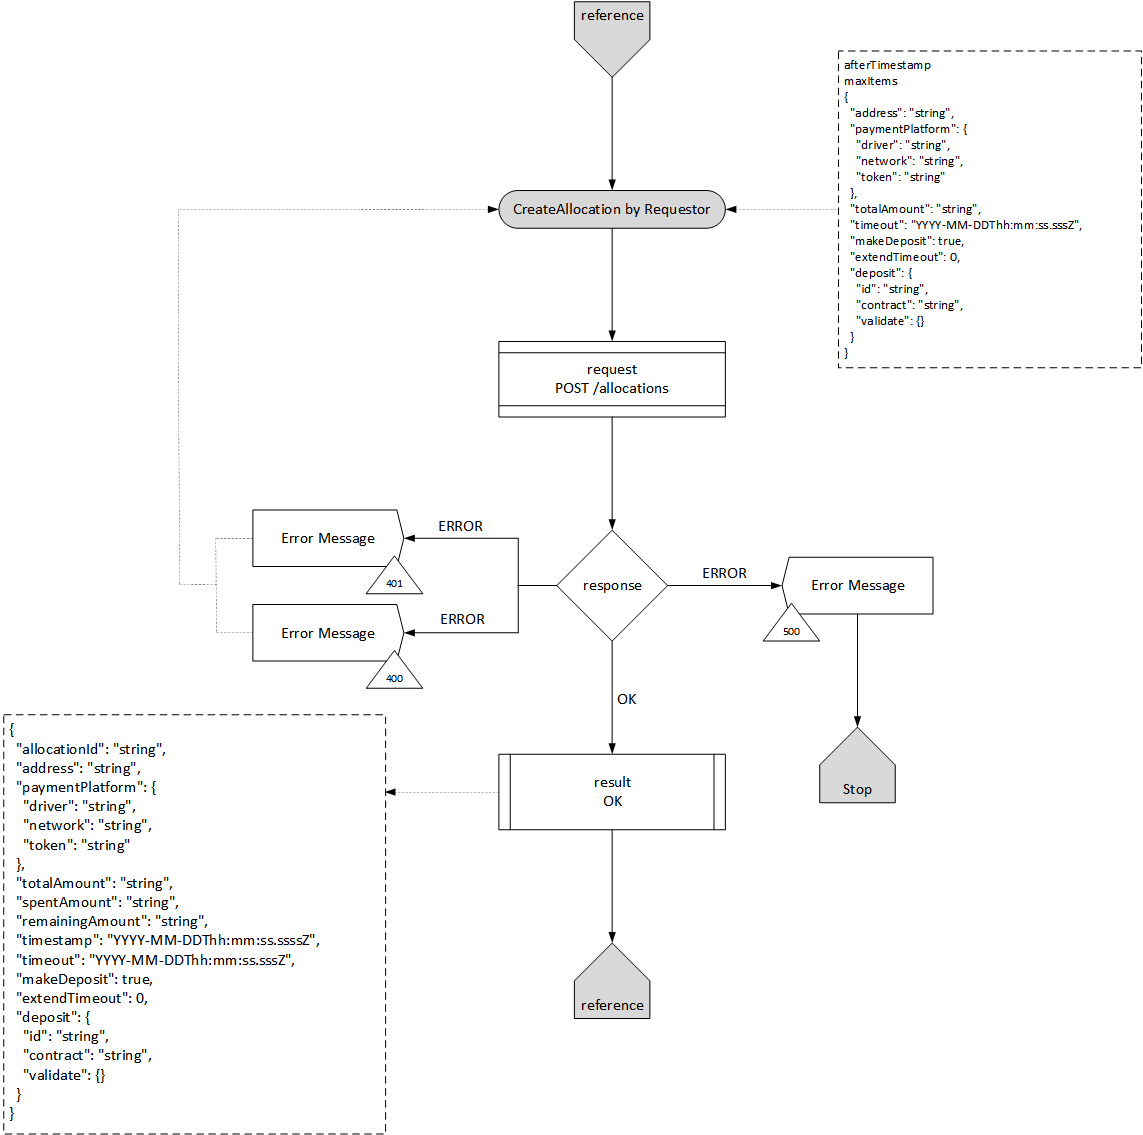
\includegraphics[width=12cm,height=12cm,angle=0]{./diag/Workflow/Payment/CreateAllocation-R-Workflow.png}
    \caption{Requestor Workflow Create Allocation Amount }
	\label{fig:RCAA}
\end{figure}


\end{enumerate}

\newpage

%% AmendAllocation

\subsubsubsubsection{AmendAllocation Function}

\begin{enumerate}

\item Profile

\begin{enumerate}

\item Description

The AmendAllocation function is used to change the Allocation Objects by Requestor Node. 
It uses the PUT /allocations/\{allocationId\} method.

An Allocation is a designated sum of money reserved for the purpose of making some particular payments. 
Allocations are currently purely virtual objects. They only exist in the Requestor node database.
An Allocation is connected to a payment account (wallet) specified by address and paymentPlatform field. 
If these fields are not present the default payment platform is used and the address is assumed 
to be identical to the Requestor's Node ID.

 
\item Side

Requestor

\end{enumerate}

\item Request

\begin{enumerate}

\item Input

\begin{tcolorbox}[boxrule=0pt, frame empty]
\begin{verbatim}

allocationId

\end{verbatim}
\end{tcolorbox}

Object
\begin{tcolorbox}[boxrule=0pt, frame empty]
\begin{verbatim}

{
  "address": "string",
  "paymentPlatform": {
    "driver": "string",
    "network": "string",
    "token": "string"
  },
  "totalAmount": "string",
  "timeout": "YYYY-MM-DDThh:mm:ss.sssZ",
  "makeDeposit": true,
  "extendTimeout": 0,
  "deposit": {
    "id": "string",
    "contract": "string",
    "validate": {}
  }
}

\end{verbatim}
\end{tcolorbox}

\begin{table}[H]
\footnotesize

\begin{center}
\begin{tabular}{|p{3cm}|l|p{3cm}|p{3cm}|p{4cm}|} 
\hline
\rowcolor{lightgray}	Name	& MO.	& Type	& Example & 	Description \\
\hline

maxItems			& O	& 	integer(\$int32)	&	10							&	Maximum number of items that server should return at once \\ 
\hline

afterTimestamp		& O &	string(\$date-time)	&	YYYY-MM-DDThh:mm:ss.sssZ	&	Apply only to records created later than the specified timestamp \\
\hline

address						& M	&	string				&								&	Address	 \\
\hline   
  
paymentPlatform. driver		& M	&	string				&								&	Payment Platform Driver \\
\hline   

paymentPlatform. network	& M	&	string				&								&	Payment Platform Network \\
\hline   
  
paymentPlatform. token		& M	&	string				&								&	Payment Platform Token \\
\hline
     
totalAmount					& M	&	string				&								&	Total Amount \\
\hline

timeout						& 	& 	string(\$date-time)	&	YYYY-MM-DDThh:mm:ss.sssZ	&	Timeout \\ 
\hline

makeDeposit					& 	& 	boolean				&	[true, false]				&	Make Deposit \\ 
\hline

extendTimeout				& 	& 	integer(\$int64)	&	0							&	Extend Timeout \\ 
\hline

deposit.id					&   & 	string				&								&	Deposit Identifier \\
\hline

deposit.contract			&   &	string				&								&	Deposit Contract \\
\hline

deposit.validate			&   &	json				&								&	Deposit Validate \\
\hline

\end{tabular}
\end{center}
\end{table}

\item REST Method

\begin{tcolorbox}[boxrule=0pt, frame empty]
\begin{verbatim} 

PUT /allocations/{allocationId}

\end{verbatim}
\end{tcolorbox}

\end{enumerate}

\item Response

\begin{table}[H]
\footnotesize

\begin{center}
\begin{tabular}{|c|l|} 
\hline
\rowcolor{lightgray}	Code 		& 	Description \\
\hline
200	 		&	OK \\
\hline
404			&	(404) The specified resource was not found. \\
\hline
401			&	(401) Authorization information is missing or invalid. \\
\hline
500			&	(500) Server error. \\
\hline
\end{tabular}
\end{center}

\end{table}

\item Result

\begin{tcolorbox}[boxrule=0pt, frame empty]
\begin{verbatim}

[
 {
  "allocationId": "string",
  "address": "string",
  "paymentPlatform": {
    "driver": "string",
    "network": "string",
    "token": "string"
  },
  "totalAmount": "string",
  "spentAmount": "string",
  "remainingAmount": "string",
  "timestamp": "YYYY-MM-DDThh:mm:ss.sssZ",
  "timeout": "YYYY-MM-DDThh:mm:ss.sssZ",
  "makeDeposit": true,
  "extendTimeout": 0,
  "deposit": {
    "id": "string",
    "contract": "string",
    "validate": {}
  }
 }
]

\end{verbatim}
\end{tcolorbox}

\begin{table}[H]
\footnotesize

\begin{center}
\begin{tabular}{|p{3cm}|l|p{3cm}|p{3cm}|p{4cm}|} 
\hline
\rowcolor{lightgray}	Name	& MO.	& Type	& Example & 	Description \\
\hline

allocationId				&	&	string				&								&	Allocation Identifier \\
\hline   

address						&	&	string				&								&	Address	 \\
\hline   
  
paymentPlatform. driver		&	&	string				&								&	Payment Platform Driver \\
\hline   

paymentPlatform. network	&	&	string				&								&	Payment Platform Network \\
\hline   
  
paymentPlatform. token		&	&	string				&								&	Payment Platform Token \\
\hline
     
totalAmount					&	&	string				&								&	Total Amount \\
\hline

spentAmount					&	&	string				&								&	Spent Amount \\
\hline

remainingAmount				&	&	string				&								&	Remaining Amount \\
\hline

timestamp					&   &	string(\$date-time)	&	YYYY-MM-DDThh:mm:ss.sssZ	&	Time of ? \\
\hline

timeout						& 	& 	string(\$date-time)	&	YYYY-MM-DDThh:mm:ss.sssZ	&	Timeout \\ 
\hline

makeDeposit					& 	& 	boolean				&	[true, false]				&	Make Deposit \\ 
\hline

extendTimeout				& 	& 	integer(\$int64)	&	0							&	Extend Timeout \\ 
\hline

deposit.id					&   & 	string				&								&	Deposit Identifier \\
\hline

deposit.contract			&   &	string				&								&	Deposit Contract \\
\hline

deposit.validate			&   &	json				&								&	Deposit Validate \\
\hline

\end{tabular}
\end{center}
\end{table}

\item Workflow

(Please see Figure ~\ref{fig:RChA} on page ~\pageref{fig:RChA}):

\begin{figure}[htbp]
    \centering
    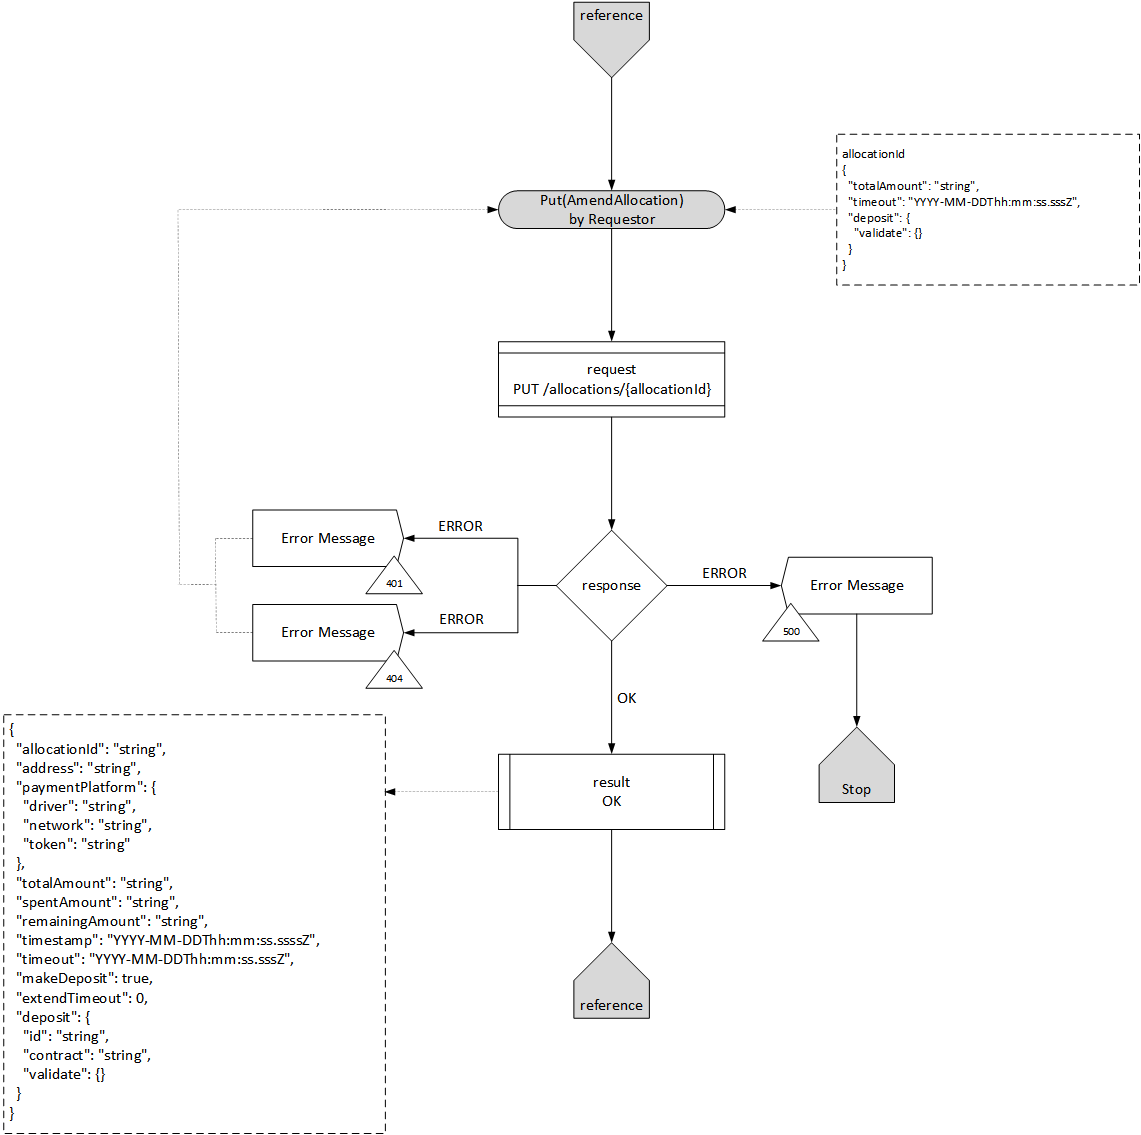
\includegraphics[width=12cm,height=12cm,angle=0]{./diag/Workflow/Payment/Put(AmendAllocation)-R-Workflow.png}
    \caption{Requestor Workflow Change (Amend) Allocation }
	\label{fig:RChA}
\end{figure}


\end{enumerate}

\newpage

%% ReleaseAmount

\subsubsubsubsection{ReleaseAllocate Function}

\begin{enumerate}

\item Profile

\begin{enumerate}

\item Description

The ReleaseAllocate function is used to release the Allocation Objects by Requestor Node. 
It uses the DELETE /allocations/\{allocationId\} method.

An Allocation is a designated sum of money reserved for the purpose of making some particular payments. 
Allocations are currently purely virtual objects. They only exist in the Requestor node database.
An Allocation is connected to a payment account (wallet) specified by address and paymentPlatform field. 
If these fields are not present the default payment platform is used and the address is assumed 
to be identical to the Requestor's Node ID.

 
\item Side

Requestor

\end{enumerate}

\item Request

\begin{enumerate}

\item Input

\begin{tcolorbox}[boxrule=0pt, frame empty]
\begin{verbatim}

allocationId

\end{verbatim}
\end{tcolorbox}

%Object
%\begin{tcolorbox}[boxrule=0pt, frame empty]
%\begin{verbatim}

%\end{verbatim}
%\end{tcolorbox}

\begin{table}[H]
\footnotesize

\begin{center}
\begin{tabular}{|p{3cm}|l|p{3cm}|p{3cm}|p{4cm}|} 
\hline
\rowcolor{lightgray}	Name	& MO.	& Type	& Example & 	Description \\
\hline

allocationId			& M	& 	string	&								&	Allocation Identifier \\ 
\hline

\end{tabular}
\end{center}
\end{table}

\item REST Method

\begin{tcolorbox}[boxrule=0pt, frame empty]
\begin{verbatim} 

DELETE /allocations/{allocationId}

\end{verbatim}
\end{tcolorbox}

\end{enumerate}

\item Response

\begin{table}[H]
\footnotesize

\begin{center}
\begin{tabular}{|c|l|} 
\hline
\rowcolor{lightgray}	Code 		& 	Description \\
\hline
200	 		&	OK \\
\hline
404			&	(404) The specified resource was not found. \\
\hline
401			&	(401) Authorization information is missing or invalid. \\
\hline
410			&	(410) Gone. \\
\hline
500			&	(500) Server error. \\
\hline
\end{tabular}
\end{center}

\end{table}

\item Result

\begin{tcolorbox}[boxrule=0pt, frame empty]
\begin{verbatim}

as above

\end{verbatim}
\end{tcolorbox}

%\begin{table}
%\footnotesize

%\begin{center}
%\begin{tabular}{|p{3cm}|l|p{3cm}|p{3cm}|p{4cm}|} 
%\hline
%\rowcolor{lightgray}	Name	& MO.	& Type	& Example & 	Description \\
%\hline

%\end{tabular}
%\end{center}
%\end{table}

\item Workflow

(Please see Figure ~\ref{fig:RRA} on page ~\pageref{fig:RRA}):

\begin{figure}[htbp]
    \centering
    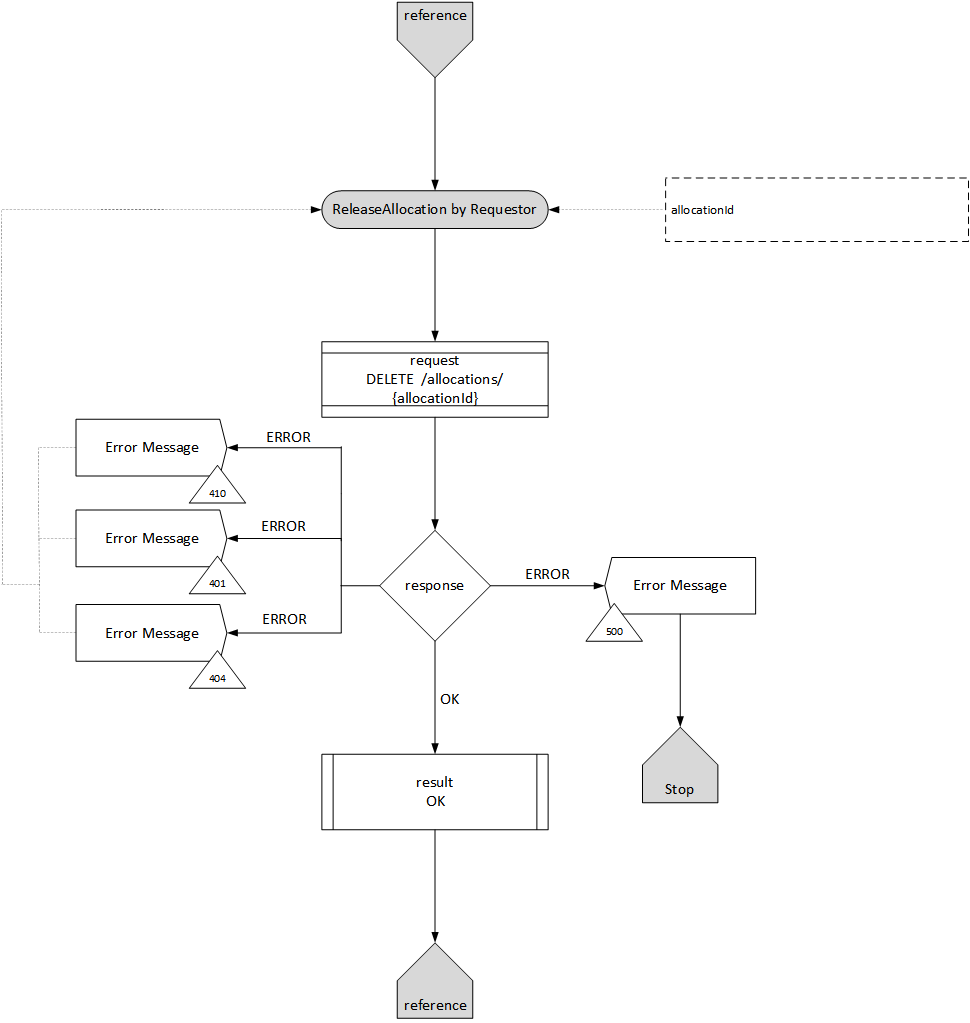
\includegraphics[width=12cm,height=12cm,angle=0]{./diag/Workflow/Payment/ReleaseAllocation-R-Workflow.png}
    \caption{Requestor Workflow Release Allocation  }
	\label{fig:RRA}
\end{figure}


\end{enumerate}

\newpage